% This file contains CHAPTER TWO

\chapter{Mathematical Background}
\label{cha:bg} 
The goal of this chapter is to provide the basic mathematical background
required for the work of this thesis. The chapter is organized by starting with
the necessary theory on hyperelliptic curves, then divisor class groups,
divisor class arithmetic and followed with standard algorithmic improvements for
computing the arithmetic. The material in this chapter is primarily taken
from~\cite{HandbookFF_2013,Galbraith_PKC_2012}.

\section{Hyperelliptic Curves}
\label{sec:hec}
In this section, theory and properties of hyperelliptic curves relevant to the
work are presented. First the definition of hyperelliptic curves is introduced,
where the three models of these curves (ramified, split and inert) are defined.
Next, necessary definitions and properties of the function field of a
hyperelliptic curve and the set of points of hyperelliptic curves (for
describing divisor class arithmetic in later sections) are presented. Then,
orders of rational functions in the function field of a hyperelliptic curve are
defined using the notion of uniformizing parameters. Finally, practical
considerations for the generic definitions of a hyperelliptic curve relative to
this work are discussed and a crucial polynomial used in split model arithmetic
is introduced.

Throughout, suppose that $k$ is a perfect field, $k[x]$ is the univariate
polynomial ring over $k$, $k(x)$ is the field of rational functions over $k$ and
$\Ck$ is a fixed algebraic closure of $k$. The leading coefficient of a polynomial
$t$ is denoted $\lcf(t)$. 

We begin by defining a hyperelliptic curve and the different models that can be
used to represent it. In order to simplify the exposition of the practical
implementations throughout this thesis, hyperelliptic curves are defined as
affine plane curves in the following. The theoretical algebraic geometry
approach generally describes hyperelliptic curves as projective plane curves
and such descriptions can be found
in~\cite{Galbraith_PKC_2012,CasselsFlynn_g2arithmetic_1996}.

\bd \label{def:heq}
\cite[Definition~12.4.1]{HandbookFF_2013} A \emph{hyperelliptic
equation} over a field $k$ is an equation of the form 
\begin{equation}
C : y^2 + h(x)y = f(x) \label{eq:heq}
\end{equation}
with $f(x), h(x) \in k[x]$ and $f(x) \not = 0$.
\ed

\br
\cite[Remark~12.4.2]{HandbookFF_2013} The curve defined by a hyperelliptic
equation (\ref{eq:heq}) is non-singular if and only if for no point $(x_0,y_0) \in \Ck \times \Ck$
on the curve that satisfies the hyperelliptic equation~\eqref{eq:heq}, both
partial derivatives vanish, i.e., $$ 2y_0 + h(x_0) = 0 \mbox{ and }
h^{\prime}(x_0)y_0 = f^{\prime}(x_0).$$
\er

\bd \label{def:hec} \cite[Definition~12.4.3]{HandbookFF_2013} A
\emph{hyperelliptic curve} $C$ of genus $g$ defined over a field $k$ is
represented by a hyperelliptic equation over $k$ that is irreducible in
$k(x,y)$, non-singular, and satisfies one of the following three conditions:
\begin{enumerate}
    \item $\deg(f(x)) = 2g + 1$ and $\deg(h(x)) \leq g$;
    \item $\deg(f(x)) \leq 2g + 1$ and $h(x)$ is monic of degree $g + 1$, or
    $\deg(f(x)) = 2g + 2$ and \begin{enumerate}
            \item either $k$ has characteristic different from 2, $\deg(h(x))
            \leq g$ and $\lcf(f(x))$ is a square in $k$,
            \item or $k$ has characteristic 2, or $h(x)$ is monic of degree
            $g+1$ and $\lcf(f(x))$ is of the form $s^2 + s$ for some $s \in
            k^*$;
            \end{enumerate}
    \item $\deg(f(x)) = 2g + 2$ and \begin{enumerate}
        \item either $k$ has characteristic different from 2, $\deg(h(x)) \leq
        g$ and $\lcf(f(x))$ is not a square in $k$,
        \item or $k$ has characteristic 2, or $h(x)$ is monic of degree $g+1$
        and $\lcf(f(x))$ is not of the form $s^2 + s$ for some $s \in k^*$.
    \end{enumerate}
\end{enumerate}

A curve $C$ is \emph{ramified} (or imaginary) in case (1), \emph{split} (or
real) in case (2), and \emph{inert} (or unusual) in case (3).
\ed

The terminology ramified, split, or inert comes from the behavior of the point
at infinity, which will be described later in Section~\ref{sec:pointsonHEC}. The
alternate terminology imaginary or real comes from analogies to quadratic number
fields. The function field of a curve, defined in the next section, has similar
properties in terms of its ideal class group and unit group to imaginary
quadratic fields if the curve model is ramified and real quadratic fields if it
is split. The alternate terminology for inert curve models (unusual) refers to
the fact that there is no number field analogue for these models. For a detailed
explanation see~\cite{HandbookFF_2013}, for example.

\be
\begin{figure}[ht]
\label{fig:hec}\centering
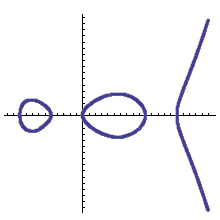
\includegraphics[scale=.75]{hec2}
\end{figure}

The ramified hyperelliptic curve $C: y^2 = x^5 -2x^4 -7x^3 + 8x^2 + 12x$ with
genus $g=2$ over $\mathbb{R}$. The curve $C$ is ramified because the degree of
$\deg(f(x)) = 2g + 1 = 5$ and $\deg(h(x)) \leq 2$.
\ee 

\subsection{Function Field of a Hyperelliptic Curve}
Important notions such as infinite points on a hyperelliptic curve and the ideal
class group of a hyperelliptic curve require the machinery presented in this
section. In the following, the coordinate ring in which the ideals of a
hyperelliptic curve live, and its members called polynomial functions, are
defined. Using the coordinate ring, function fields of a hyperelliptic curve and
their members, called rational functions, are defined. The section concludes by
defining conjugates of polynomials and rational functions, as these are required
to describe unique representations of both, and used when evaluating rational
functions on points at infinity. For more details, the reader is referred
to~\cite{MenezesWuZuccherato_elementary_1996}.


\bd \label{def:coordring}
\cite[Definition~8]{MenezesWuZuccherato_elementary_1996} The \emph{coordinate
ring} of $C$ over $k$, denoted $k[C],$ is the quotient ring 
$$ k[C] = k[x,y]/(y^2 + h(x)y - f(x)),$$ where $(y^2 + h(x)y - f(x))$ denotes
the ideal in $k[x,y]$ generated by the polynomial $y^2 + h(x)y - f(x)$.
Similarly, the coordinate ring of $C$ over $\Ck$ is defined as $$ \Ck[C] =
\Ck[x,y]/(y^2 + h(x)y -f(x)).$$ Elements of $k[C]$ and $\Ck[C]$ are called
\emph{polynomial functions} on $C$.
\ed

Every polynomial function $G(x,y)\in \Ck[C]$ is represented as $G(x,y) = a(x) -
b(x)y,$ where $a(x),b(x) \in \Ck[x]$, are unique. The unique representation is
obtained by replacing $y^2$ by $f(x) - h(x)y$ repeatedly wherever $y^2$ occurs.

\bd \label{def:functionfield}
\cite[Definition~13]{MenezesWuZuccherato_elementary_1996}  The field of
fractions of $k[C]$ is called the \emph{function field} of $C$ over $k$ and is
denoted by $k(C)$. Similarly, the function field $\Ck(C)$ of $C$ over $\Ck$ is
the field of fractions of $\Ck[C]$. Elements of $k(C)$ and $\Ck(C)$ are called
\emph{rational functions} on $C$.
\ed

Definitions relating to unique representations of rational functions and their
conjugates are presented in the following.

\bd\label{def:polyconj} 
\cite[Adapted from Definition~10]{MenezesWuZuccherato_elementary_1996} Let
$G(x,y) = a(x) - b(x)y$ be a polynomial function in $\Ck[C]$. The conjugate of
$G(x,y)$ is defined to be the polynomial function $\overline{G}(x,y) = a(x) +
b(x)(h(x) + y)$.
\ed

\bl\label{lem:conjmul}
\cite[Adapted from Lemma~12]{MenezesWuZuccherato_elementary_1996} For a
polynomial function $G \in \Ck[C]$, we have $G\overline{G} \in \Ck[x]$.
\begin{proof}
    Let $G = a(x) - b(x)y$, then $\overline{G}(x,y) = a(x) + b(x)(h(x) + y)$ and 
    $$ G\overline{G} = a^2(x) + a(x)b(x)h(x) - b^2(x)(y^2 + yh(x)) = a^2(x) -
    a(x)b(x)h(x) - b^2(x)f(x) \in \Ck[x].$$
\end{proof}
\el

\bl\label{lem:ratform}
A rational function $R \in \Ck(C)$ can be written as $R = s(x) - t(x)y$ where $
s,t \in \Ck(x).$
\begin{proof}
    Let $R = G/H$, for $G,H \in \Ck[C]$. Let $c(x) = H\overline{H}$ by
    Lemma~\ref{lem:conjmul}. Suppose that $G\overline{H} = a(x) - b(x)y$ with
    $a(x),b(x) \in \Ck[x]$, then $R = s(x) + t(x)y$ with $s(x) = a(x)/c(x) \in
    \Ck(x)$ and $t(x) = b(x)/c(x) \in \Ck(x)$.
\end{proof}
\el

\bd\label{def:ratconj}
For a rational function $R = s(x) - t(x)y$ with $s(x),t(x) \in \Ck(x)$, the
conjugate of $R$ is defined as the rational function $\overline{R} = s(x) +
t(x)(h(x) + y)$, and $R,\overline{R} \in \Ck(C).$
\ed



\subsection{Points on a Hyperelliptic Curve}\label{sec:pointsonHEC}
In Section~\ref{sec:dcg} the ideal class group of a hyperelliptic curve $C$ is
defined using properties of the set of points on $C$.  In this section finite
and infinite points along with their sets are defined, then the hyperelliptic
involution and its properties relevant to the work is discussed.

\bd \label{def:finset}
\cite[Adapted from Definition~12.4.8]{HandbookFF_2013} Let $C$ be a
hyperelliptic curve over the field $k$. For any extension field $L$ of $k$, the
set of \emph{finite points} on $C$ defined over $L$ is the set of solutions
$(x_0,y_0) \in L \times L$ to the hyperelliptic equation \eqref{eq:heq}.
\ed

\bd \label{def:rationalvalue}
\cite[Definition~14]{MenezesWuZuccherato_elementary_1996}  Let $R \in
\Ck(C)$, and let $P$ be a finite point on $C$. Then the rational function
$R$ is  defined at $P$ if there exist polynomial functions $G,H \in \Ck[C]$
such that $R = G/H$ and $H(P) \neq 0$; otherwise, $R$ is not defined
at $P$. If $R$ is defined at $P$, the value of $R$ at $P$ is defined
to be $R(P) = G(P)/H(P).$
\ed

\bd \label{def:zeropole}
\cite[Adapted from Definition~18]{MenezesWuZuccherato_elementary_1996}  Let $R
\in \Ck(C)^{\ast}$ be a rational function, and let $P$ be a point on $C$.
The point $P$ is said to be a \emph{zero} of $R$ if $R(P) = 0$. The function $R$
is said to have a \emph{pole} at $P$ if $R$ is not defined at $P$.
\ed


\bd \label{def:infpoint} \cite[Adapted from Definition~12.4.7]{HandbookFF_2013}
Let $C$ be a hyperelliptic curve over a field $k$ with hyperelliptic equation as
described in Definition~\ref{def:heq}. The poles of the rational function $x \in
\Ck(C)^{\ast}$ are called the points at infinity on $C$.
\ed

\bd\label{def:infpoints}
\cite[Adapted from Definition~10.1.16]{Galbraith_PKC_2012}
Points at infinity on the associated hyperelliptic curve lie on the projective
plane $P^2(k)$ and are denoted $\pp = (1 : \ap : 0)$ and $\pn = (1 : \an : 0)$
in weighted projective coordinates, where $\ap$ and $\an$ are particular
constants in $k$ depending on  the hyperelliptic equation used to represent the
curve. Conditions on $\ap$ and $\an$ for each model go as follows:
\begin{itemize}
    \item $\ap,\an \in k$ for split models,
    \item $\alpha = \ap = \an$, $\alpha \in k$ for ramified models and,
    \item  $\ap,\an \not \in k$ but $\ap,\an$ in a quadratic extension of $k$ for inert models.
\end{itemize}
Explicit values for $\ap,$ $\an$ are given in Definition \ref{def:apan}.
\ed


\bd \label{def:infset}
\cite[Adapted from Definition~12.4.8]{HandbookFF_2013}  Let $C$ be a
hyperelliptic curve over the field $k$. For any extension field $L$ of $k$, the
\emph{set of infinite points} on $C$ defined over $L$ is the set
\begin{equation}
    S =
      \begin{cases}
        \{ \infty = \pp = \pn \} & \text{if $C/L$ is ramified,}\\
        \{ \pp, \pn \} & \text{if $C/L$ is split,}\\
        \emptyset & \text{if $C/L$ is inert.}
      \end{cases}       
  \end{equation}
\ed

\bd \label{def:setofpoints}
\cite[Adapted from Definition~12.4.8]{HandbookFF_2013}  The set of finite points
defined in Definition~\ref{def:finset}, and set of infinite points defined in
Definition~\ref{def:infset} together form the set of \emph{points of $C$ defined
over $L$} or the set of \emph{$L$-rational points of $C$}, denoted by $C(L)$.
\ed

\be\label{ex:ramified} Let $C : y^2 + (3x^2 + 1)y = x^5 + 4x + 1$ be
hyperelliptic curve over $\F_5$. Then by Definition~\ref{def:infset} $C$ is a
ramified and $C(\F_5) = \{(\infty), (0,2),(1,3),(4,3)\}$. All finite points
produce an equality within the hyperelliptic equation with $(a,b) \rightarrow (x,y)$.
For the point at infinity, this can be seen via a projective coordinate
representation $(x,y,z) = (1,0,0) = \infty$, where the weighted projective
hyperelliptic equation is $C := y^2 + (3x^2z + z^3)y = zx^5 + 4xz^5 + z^6$ and
finite points are represented as $(x,y,1)$.
\ee

\be\label{ex:inertsplit} Let $C : y^2 = 2x^6 + 2x^4 + 2x^2 + 2$ be a
hyperelliptic curve of genus 2 defined over the finite field $\F_{3}$, then
$C(\F_{3}) = \emptyset$ so $C$ has no points over $\F_{3}$ and is inert by
Definition~\ref{def:setofpoints}.
\ee 
 

In the following, properties of hyperelliptic points are discussed, starting
with the definition of the hyperelliptic involution, an important morphism on
the set of $\Ck$-rational points of a hyperelliptic curve.

\bd \label{def:involution}
\cite[Adapted from Definition~12.4.9]{HandbookFF_2013}  The \emph{hyperelliptic
involution} of a hyperelliptic curve $C$ defined over $k$ is the map $\iota :
C(\Ck) \rightarrow  C(\Ck)$ that sends a finite point $P = (x_0,y_0)$ of $C$ to
the point $\OP = (x_0, -y_0 - h(x_0))$ of $C$. If $C$ is ramified, then
$\iota(\infty) = \infty$. If $C$ is split, then $\iota(\pp) = \pn$ and
$\iota(\pn) = \pp$.
\ed

\br
Conjugates of polynomial and rational functions defined in
Definitions~\ref{def:polyconj} and~\ref{def:ratconj} are extensions of the
hyperelliptic involution to the set of polynomial and rational functions over
$C$, respectively.
\er

\bd \label{def:rampoint}
\cite[Adapted from Remark~12.4.10]{HandbookFF_2013}  A point $P$ on a
hyperelliptic curve $C$ is ramified (or special) if $\iota(P) = P$, i.e, $P =
\OP$, and unramified (or ordinary) otherwise. 
\ed

\be
By Definition~\ref{def:rampoint}, the point at infinity $\infty$ on a ramified
model hyperelliptic curve is ramified since $\iota(\infty) = \infty$. The points
at infinity $\pp,$ $\pn$ on a split model hyperelliptic curve are unramified
because $\iota(\pp) = \pn$ and vice versa.
\ee

\be
By Definition~\ref{def:rampoint}, all points $P$ in Example~\ref{ex:ramified}
have the property that $\iota(P) = P$ and are therefore ramified. 
\ee





\subsection{Orders of Rational Functions}\label{sec:orders}
In Section~\ref{sec:dcg}, the definition of a principal divisor as the divisor
defined by a rational function requires the order (or valuation) of that rational function at
the $\Ck$-rational points. In this section, the order of rational functions at a
rational point is defined using the notion of uniformizing parameters. The
degree of rational functions used to define the order requires discussion of
Puiseux expansions and are presented first.

\bd\label{def:Puiseux} \cite[Adapted from Section 2]{jacobson_fast_2007} A
(non-zero) \emph{Puiseux series} in an indeterminate $t$ over a field $k$ is an
infinite series of the form $\sum_{i = -\infty}^d a_it^i$ where $d \in \Z,$
$a_i \in k$ for $i \leq d$, and $a_d \neq 0$. The
non-zero Puiseux series in $t$ over $k$ together with 0, form a field denoted by
$k \la t^{-1} \ra $.
\ed

\br\label{rem:Puiseux}
\cite[Adapted from Section 2]{jacobson_fast_2007} Consider the hyperelliptic curve $C :
y^2 + h(x)y = f(x)$ defined over $k$.
\begin{itemize}
    \item If $C$ is ramified, then $y$ and $y+h$ are Puiseux series in
    $x^{-1/2}$ with coefficients in $k$. 
    \item If $C$ is split, then $y$ and $y+h$ are Puiseux series in $x^{-1}$
    with coefficients in $k$.
    \item If $C$ is inert, then $y$ and $y+h$ are Puiseux series in $x^{-1}$
    with coefficients in a quadratic extension of $k$, but not in $k$.
\end{itemize} 
\er

\be
Consider a hyperelliptic curve $C : y^2 = f(x)$ over $k$. Then $y = \sqrt{f(x)}$
and there are two roots, $\sqrt{f(x)}$ and $-\sqrt{f(x)}$. If a square root $y$
of $f(x)$ is explicitly extracted, then $y$ has a Puiseux expansion over $k$ in
$x^{-1/2}$ when $C$ is ramified, and in $x^{-1}$ when $C$ is split.
\ee

The existence of a Puiseux series for $y$ implies that every element of the
coordinate ring $k[C]$, and hence the function field $k(C)$, has a Puiseux
expansion over $k$ in $x^{-1/2}$ for ramified models, and two in $x^{-1}$ for
split models depending on the embedding of $k(C)$ in $k<x^{-1}>$. Fixing such an
embedding is discussed in Lemma \ref{lem:explicituni}.

\bd\label{def:degR}
\cite[Adapted from Section 3]{jacobson_fast_2007} Let $R \in k(C)$. The degree of $R$ is
the largest power of $x$ in $R$ considered as a Puiseux series in $x^{-1}$ for
both split models and inert models, and in $x^{-1/2}$ for ramified models. The degree of a
rational function $R$, denoted $\deg(R)$, is a half integer for ramified models
and an integer for split models.
\ed

Definition~\ref{def:rationalvalue} describes what it means for a rational
function to be defined at a finite point on a hyperelliptic curve $C$. The
following completes the picture for infinite points on $C$.

\bd\label{def:infratval}
\cite[Adapted from Definition~17]{MenezesWuZuccherato_elementary_1996} Let $C$
be a hyperelliptic curve over $k$ and $R \in k(C)$ be a rational function. If
$C$ is ramified then \begin{enumerate}
    \item $R(\infty) = 0 $ if $\deg(R) < 0$.
    \item $R$ is undefined at $\infty$ if $\deg(R) > 0$.
    \item $R(\infty)$ is the constant coefficient of $R$ if $\deg(R) = 0$.
\end{enumerate} If $C$ is split, then $R(\pp)$ is defined analogously to
$R(\infty)$ in ramified models and $R(\pn) = \overline{R}(\pp)$, where
$\overline{R}$ is the conjugate of $R$.
\ed

In the rest of this section, orders of rational functions at points and their properties
are defined using uniformizing parameters. Intuitively the order of a function
$R \in \Ck(C)$ at a point $P$ is the measure of the multiplicity of the
intersection of the curve $C$ with $R$.  First uniformizing parameters are
defined, then the order of a polynomial function at a point and its properties,
followed by the order of a rational function at point and explicit unifying
parameters for each possible type of point.

\bd\label{def:uniformizing}
\cite[Adapted from Definitions~23 and~24]{MenezesWuZuccherato_elementary_1996} Let $P$
be a $\Ck$-rational point on the hyperelliptic curve $C$. Then there exists a
function $U \in \Ck(C)$ with $U(P) = 0$ such that the following property holds:
for each function $R$ in $\Ck(C)^*$, there exists an integer $d$ and a
rational function $S \in \Ck(C)$ such that $P$ is neither a zero nor a pole of
$S$, and $R  = U^dS$. Furthermore, the number $d$ does not depend on the choice
of $U$. The function $U$ is called a \emph{uniformizing parameter} for $P$. The
integer $d$ is called the order of $R$ at $P$ and is denoted by $d =
\ord_P(R)$.
\ed


\bl \label{lem:orderproperties} \cite[Adapted from Lemmas~25
and~28]{MenezesWuZuccherato_elementary_1996}  Let $G_1,G_2 \in \Ck[C]^{\ast}$
and $P \in C$, and let $\ord_P(G_1) = r_1,$ $\ord_P(G_2) = r_1$ then, 
\begin{enumerate}
\item $\ord_P(G_1G_2) = \ord_P(G_1) + \ord_P(G_2).$
\item Suppose that $G_1 \neq -G_2.$ If $r_1 \neq r_2$ then $\ord_P(G_1 + G_2) =
\min(r_1,r_2).$ If $r_1 = r_2$ then $\ord_P(G_1 + G_2) \geq \min(r_1,r_2).$
\item $\ord_P(G_1) = \ord_{\overline{P}}(\overline{G_1})$.
\end{enumerate}
\el

\bt \label{thm:polyfinite} 
\cite[Theorem~29]{MenezesWuZuccherato_elementary_1996}  Let $G \in
\Ck[C]^{\ast}.$ Then $G$ has a finite number of zeros and poles. Moreover, 
$$ \sum_{P \in C} \ord_P(G) = 0.$$
\et

\bd \label{def:rationalorder}
\cite[Definition~30]{MenezesWuZuccherato_elementary_1996}  Let $R = G/H \in
\Ck(C)^{\ast}$ and $P \in C$. The order of $R$ at $P$ is defined to be
$\ord_P(R) = \ord_P(G) - \ord_P(H).$
\ed

\bt\label{thm:ratfinite} 
\cite[Adapted from Theorems~7.7.1 and~7.7.11]{Galbraith_PKC_2012} Let $C$ be a
hyperelliptic curve over $k$ and $R \in \bar{k}(C)^*$ a rational function. Then
$R$ has finitely many poles and zeros. Moreover, $$ \sum_{P \in C} \ord_P(R) =
0.$$
\et


\bl \label{lem:explicituni}
\cite[Adapted from Lemmas 10.1.21 and 10.1.22]{Galbraith_PKC_2012} Let $P =
(x_P,y_P) \in C(k)$ be a point on the hyperelliptic curve $C$ over $k$. Then the
explicit uniformizing parameter for \begin{itemize}
  \item an unramified finite point $P = (x_P,y_P)$ is the function $x - x_P$ and
  $\ord_P(x-x_P) = 1$,
  \item a ramified finite point $P = (x_P,y_P)$ is the function $y - y_p$ and
  $\ord_P(x-x_P) = 2$,
  \item an unramified infinite point $\pp$ is the function $1/x$ and for
  rational function $R$, $\ord_{\pp}(R) = -\deg(R)$ and $\ord_{\pn}(R) =
  -\deg(\overline{R})$,
  \item a ramified infinite point $\infty$ is the function $y/x^{g+1}$ and for
  rational function $R$, $\ord_{\infty}(-2\deg(R))$.
\end{itemize}
\el

\subsection{Practical Considerations}\label{sec:practicalConsiderations}
Not all hyperelliptic curve models defined in Definition~\ref{def:hec} are
practical for divisor class arithmetic. Inert models are cumbersome to work with
and only exist for small field sizes relative to the genus. Moreover, the
hyperelliptic equation for split models as defined in Definition \ref{def:hec} has
more than one form over characteristic 2 fields. These issues are addressed in
this section.

In the following theorem, transformations of hyperelliptic curve models are
discussed in order to address the problem with inert curves. Arguments for the
inefficiency and scarcity of inert hyperelliptic curves are provided, with the
conclusion that inert models are impractical and not necessary for most
applications. Following, a unified form for the hyperelliptic equation of split
hyperelliptic curve that aligns with efficient arithmetic techniques is
discussed.

\bt\label{thm:transform} \cite[Adapted from Theorem~12.4.12]{HandbookFF_2013}
Let $C$ be a hyperelliptic curve of genus $g$ over a field $k$ as defined in
Definition \ref{def:heq}, and let $x_0,y_0 \in k$. Substituting  $$ x = t^{-1} +
x_0, \text{ and } y = \frac{bz}{t^{g+1}} + a $$ into (\ref{def:heq}), with 
\begin{equation}
    a =
      \begin{cases}
        y_0 & \text{ if char}(k) = 2\\
        -h(x_0)/2 & \text{ otherwise,}
      \end{cases}       
  \end{equation}
and
\begin{equation}
    b =
      \begin{cases}
        1 & \text{ if $h(x_0) + 2y_0 = 0$,}\\
        h(x_0) + 2y_0 & \text{ otherwise,}
      \end{cases}       
  \end{equation}
yields a hyperelliptic curve $C^{\prime} : z^2 + H(t)z = F(t)$ of genus $g$ over
$k$ where $$H(t) = b^{-1}t^{g + 1}(h(t^{-1} + x_0) + 2a), \mbox{ } F(t) =
b^{-2}t^{2g + 2} (f(t^{-1} + x_0) - ah(t^{-1} + x_0) - a^2),$$
and the following conditions hold:
\begin{enumerate}
    \item If $P = (x_0,y_0)$ is a finite ramified point on $C$, then
    $C^{\prime}$ is a ramified hyperelliptic curve.
    \item If $P = (x_0,y_0)$ is a finite unramified point on $C$, then
    $C^{\prime}$ is a split hyperelliptic curve.
    \item If no finite point on $C$ has $x$-coordinate $x_0$ then
    $C^{\prime}$ is an inert hyperelliptic curve.
\end{enumerate}
\et

Recall that the model used to represent a hyperelliptic curve determines the
number and type of points at infinity.  A split model representation has two
$k$-rational points at infinity, denoted $\pp$ and $\pn = \overline{\pp}$.
Ramified models have a single ramified $k$-rational point at infinity, and inert
models have none.  It is sometimes possible to change the model of a curve $C$
without modifying the field of definition $k$ by translating other points to
infinity. If $C$ has a ramified $k$-rational point, one can obtain a ramified
model for $C$ via translation of this point to infinity, by
Theorem~\ref{thm:transform}. If $C$ has a split $k$-rational point, then
similarly, that point can be translated to infinity, providing two points at
infinity $\pp$, $\pn$ and thus $C$ can be represented with a split model. If no
$k$-rational points exists, including at infinity, then the hyperelliptic curve
$C$ is inert and no alternative ramified or split models are possible over $k$.
However, hyperelliptic curves that have neither a ramified nor an unramified
$k$-rational point are rare and only exist over fields whose cardinality is
small relative to the genus. If $k$ is a finite field of cardinality $q$, the
Weil bound $\#C(k) \geq q + 1 - 2g \sqrt{q}$ guarantees that a genus $g$
hyperelliptic curve $C$ over $k$ has a $k$-rational point whenever $q > 4g^2$,
and an unramified $k$-rational point when $q > 4g^2 + 2g + 2$~\cite{Sutherland_g3_2019}.  

\be \label{ex:g2Weil}
Let $C$ be a hyperelliptic curve over $k$ with $g = 2$. The Hasse-Weil bound
implies that for any field $k$ with cardinality greater than $4(2)^2 = 16$, $C$
has at least one $k$-rational point, and therefore at worst admits a split
model. 
\ee

Inert hyperelliptic curves have been shown to have less efficient
arithmetic than the other models~\cite{RozenhartJacobsonScheidler_Tabulation}
and can easily be avoided in practice by translating to a
split or ramified model when $q$ is sufficiently large to guarantee a
$k$-rational point, or by considering the curve as a split model over a
quadratic extension of $k$ otherwise. Thus, in this work we only consider
hyperelliptic curves given by a ramified or split model.

\be\label{ex:quadraticext}
Let $\F_{3^2} = \F_3[t]/(t^2 + t + 2)$, and let $\alpha$ be a root of the
primitive polynomial $t^2 + t + 2$ in $\F_3$. The powers of $\alpha$ are:

\begin{table}[ht]\label{tab:f9}
\[ \begin{array}{|c||c|c|c|c|c|c|c|c|} 
  \hline
  n&0&1&2&3&4&5&6&7\\ \hline

  \alpha^n &1&\alpha&2\alpha+1&2\alpha+2&2&2\alpha&\alpha+2&\alpha+1\\  \hline
\end{array} \]
\end{table}

Let $C : y^2 = 2x^6 + 2x^4 + 2x^2 + 2$ be defined as in
Example~\ref{ex:inertsplit}, and recall that $C$ is inert over $\F_{3}$ since it
has no $\F_{3}$-rational points. Consider $C$ over $\F_{3^2}$ instead, then $C$
is split by Definition~\ref{def:hec} because the leading coefficient of $f(x)$
is $2 = (2\alpha + 1)^2$, so it is a square in $\F_{3^2}$. Furthermore,
$C(\F_{3^2}) = \{\pp, \pn, (0,\alpha^2), (0,\alpha^6), (1,\alpha^2),
(1,\alpha^6), (\alpha,0), (\alpha^2,0), (\alpha^3,0),\\ (2,\alpha^2),
(2,\alpha^6), (\alpha^5,0), (\alpha^6,0), (\alpha^7,0) \}$.
\ee

In split hyperelliptic curve arithmetic, it is practical to only consider one
form of the hyperelliptic equation of a curve and design the algorithms based on
properties of that equation. Over fields of characteristic other than 2, the
$f$ polynomial of the hyperelliptic equation (\ref{def:heq}) has degree $2g +
2$. The following theorem shows that any split hyperelliptic curve over
characteristic 2 fields can be transformed into a curve with the degree of
$\deg(f) = 2g +2$ as well. 

\bt
Let $C : y^2 + h(x)y = f(x)$ be a split hyperelliptic curve over a perfect field
$k$ of characteristic 2 and cardinality greater than 2 with $\deg(f) < 2g + 2$
and $h(x)$ monic with degree $g + 1$ as defined in (\ref{def:hec}). Then $C$ can
be transformed to a split hyperelliptic curve $C^{\prime} : Y^2 + h(x)Y = F(x)$
where $\deg(F(x)) = 2g + 2$ and the leading coefficient of $F(x)$ is of the form
$e^2 + e$ with $e \in k^*.$
\begin{proof}
  Let $e \in k$ where $e^2 + e \neq 0$, so $e \neq 1$. Let $Y = y +
  ex^{g+1}$. Then, \begin{eqnarray*}
    y^2 + h(x)y - f(x) &=& (Y + ex^{g+1})^2 + (Y + ex^{g+1})h(x) - f(x)\\
                       &=& Y^2 + h(x)y + e^2x^{2g + 2} + eh(x)x^{g+1} - f(x)\\
                       &=& Y^2 + h(x)y - F(x),\\
  \end{eqnarray*}
for $F(x) =  e^2x^{2g + 2} + eh(x)x^{g+1} - f(x)$. Notice $F(x) \in
k[x]$, $\deg(F(x)) = 2g + 2$, and the leading coefficient of $F(x)$ is
$e^2 + e$ since  $\deg(f(x)) < 2g + 2$, $\deg(h(x)) = g + 1$ and $h(x)$ is
monic. Therefore, $C^{\prime} : Y^2 + h(x)Y = F(x)$ is a split hyperelliptic
curve with the desired form.
\end{proof}
\et

Going forward, only split models with $\deg(f(x)) = 2g + 2$ will be considered.
Next, a polynomial $\Vp(x)$ crucial for arithmetic on hyperelliptic curves with
a split model is described. The polynomial $\Vp(x)$ is essentially a function
that cancels the pole of $y$ at $\pp$ for a hyperelliptic curve $C : y^2 + h(x)y
= f(x)$. Its conjugate $\Vn(x) = -\Vp(x) - h(x)$ similarly cancels the pole of
$y$ at $\pn$. Recall from Definition~\ref{def:infpoints} that $\pp = (1:\ap:0)$
and $\pn = (1:\an:0)$. The values $\ap$ and $\an$ are explicitly defined in
Definition~\ref{def:apan} and the polynomials $\Vp$ and $\Vn$ are defined in
Definition~\ref{def:vpvn}.

\bd \label{def:apan} \cite[Adapted from Excercise~10.1.28]{Galbraith_PKC_2012}
Let $C : y^2 + h(x)y = f(x)$ be a split model hyperelliptic curve over $k$ of
genus $g$. Define $\ap, \an \in k$ to be the roots of $Y^2 + h_{g+1}Y - f_{2g +
2}$ where $h_{g+1}$ and $f_{2g + 2}$ are the coefficients of $x^{g+1}$ and
$x^{2g +2}$ of $h(x)$ and $f(x)$ respectively.
\ed

\be
Let $C$ be defined as in Example~\ref{ex:quadraticext}. The roots of $Y^2 +
h_{g+1}Y - f_{2g + 2} = Y^2 - 2$ are $\alpha^2$ and $\alpha^6$. Then by
Definition~\ref{def:apan}, the points at infinity defined over $F_{3^2}$ are
explicitly defined as $\pp = (1 : \alpha^2 : 0)$ and $\pn = (1 : \alpha^6 :0)$
satisfying the weighted projective model $C_W : y^2 = 2x^6 + 2x^4z^2 + 2x^2z^4 +
2z^6$ since $2 = \alpha^4$, so both $(\alpha^2)^2 = \alpha^4 = 2$ and
$(\alpha^6)^2 = \alpha^{36} = \alpha^4 = 2$.
\ee

\bd \label{def:vpvn} \cite[Adapted from Excercise~10.1.28]{Galbraith_PKC_2012}
Let $C : y^2 + h(x)y = f(x)$ be a split model hyperelliptic curve over $k$ of
genus $g$. Let $\ap, \an \in k$ as described in Definition \ref{def:apan}, then
there exists a polynomial $ \Vp(x) =\ap x^{g+1} + \cdots \in k[x]$ such that
$\deg(\Vp(x)^2 + h(x)\Vp(x) - f(x)) \leq g$. Similarly, there exists a
polynomial $\Vn(x) =\an x^{g+1} + \cdots \in k[x]$ such that $\deg(\Vn(x)^2 +
h(x)\Vn(x) - f(x)) \leq g$. Furthermore, $\Vn(x) = -\Vp(x) - h(x)$.
\ed

The computation of $\Vp(x)$ is described in Algorithm~\ref{alg:vp},
where $\Vn(x)$ can be computed similarly starting with $\an$ or as $\Vn(x) =
-\Vp(x) - h(x)$. A brief explanation follows, since the choice of leading
coefficient already implies that $\deg(\Vp(x)^2 + h(x)\Vp(x) - f(x)) \leq 2g +
1$, the idea is to solve linear equations in the coefficients $\Vp_{g}$,
$\Vp_{g-1}, \Vp_{g-2}, ...,\Vp_{0}$ iteratively, with $\deg(\Vp(x)^2 +
h(x)\Vp(x) - f(x))$ decreasing by one in every iteration. 

\begin{algorithm}[ht]
  \caption{Compute $\Vp$}
  \label{alg:vp}
  {\fontsize{12}{18}\selectfont
  \begin{algorithmic}[1]
  \Require $f,$ $h,$ $g.$
  \Ensure $\Vp$ polynomial such that $\deg(f -\Vp(\Vp + h)) \leq g$ for genus $g$.
  \vspace{5pt}
  \State Let $h_{g+1}$ be the $g+1$ coefficient of $h$. \hspace{150pt} \emph{// can be zero}
  \State Let $f_{2g+2}$ be the $2g +2$ coefficient of $f$. 
  \State Let $\Vp_{g+1}$ be the positive solution $\ap$ to the equation $f_{2g+2} - x(x + h_{g+1})$.
  \State $\Vp = \Vp_{g+1}x^{g+1}$.
  \State $d = (2\Vp_{g+1} + h_{g+1})^{-1}$.
  \State Let $i = g$.
  \While{$i \geq 0$}
    \State $\Vp_{g+1+i} =$ $g+ 1 + i$ coefficient of $f - \Vp(\Vp + h)$.
    \State $\Vp = \Vp + d(\Vp_{g+1+i}x^i)$
    \State $i = i - 1$.
  \EndWhile
  \State \Return $\Vp$.
  \end{algorithmic}
  }
\end{algorithm}

\newpage


\section{Divisor Class Group}\label{sec:dcg}
Unlike the case of elliptic curves, the points on a hyperelliptic curve defined
over any extension field of $k$ do not form an abelian group. Instead one needs
to use divisors, where a divisor is a formal sum of points. The set of all
divisors over a hyperelliptic curve forms an abelian group under addition, in
which important subgroups can be used to form a quotient group called the
divisor class group. The divisor class group of a hyperelliptic curve has many
practical uses, and its definition is the main goal of this section. For more
information on divisors and the divisor class group, the reader is referred
to~\cite[Section~7.6]{Galbraith_PKC_2012}. In the following, a series of
definitions and properties related to divisors are presented, finishing with a
definition of the divisor class group.


\bd
\cite[Adapted from Definition~7.6.1]{Galbraith_PKC_2012} Let $C$ be a
hyperelliptic curve over $k$. A \emph{divisor} on $C$ is a formal sum 
\begin{equation}\label{eq:divisor}
  D = \sum_{P \in C(\Ck)} n_P(P)
\end{equation}
where $n_P \in \mathbb{Z}$ and only finitely many $n_P \neq 0$. The integer
$n_P$ is called the order of $D$ at $P$, written as $\ord_P(D) = n_P$.
\ed

\bd\label{def:support}
\cite[Adapted from Definition~7.6.1]{Galbraith_PKC_2012} The \emph{support} of
the divisor $D$ in equation (\ref{eq:divisor}) is $ \supp(D) = \{ P \in C(\Ck) :
n_P \neq 0 \}.$
\ed

\be\label{ex:divisors} 
Let $C : y^2 = x^6 + 5x^5 + 3x^4 + x + 2$ be a hyperelliptic curve over
$\F_{7}$, then  $C(\F_{7}) = \{\pp, \pn, (0,4), (0,3), (3,1), (3,6), (4,1),
(4,6), (5,1), (5,6), (6,0)\}$. The following are divisors on $C$:
\begin{itemize}
  \item $D_1 = \pp + \pn$ with $\supp(D_1) = \{\pp,\pn\}$.
  \item $D_2 = 2(0,4) - 2(0,3)$ with $\supp(D_2) = \{(0,4),(0,3)\}$.
  \item $D_3 = (5,6) + (3,1) + 5(4,1)$ with $\supp(D_3) = \{(5,6),(3,1),(4,1)\}$.
  \item $D_4 = (4,6) - \pp$ with $\supp(D_4) = \{(4,6), \pp\}$.
  \item $D_5 = (6,0)$ with $\supp(D_5) = \{(6,0)\}$.
\end{itemize}
\ee

\bd\label{def:affinediv}
\cite[Adapted from Definition~10.3.1]{Galbraith_PKC_2012} Let $C$ be a
hyperelliptic curve over $k$. Let $S$ be the set of infinite points on $C$,
i.e., $S = \{\infty \}$ if $C$ is ramified and $S = \{\pp, \pn\}$ if
$C$ is split. A divisor $D$ is an \emph{affine divisor} on $C$ if $\supp(D) \cap
S = \emptyset$.
\ed

\be
Consider the divisors $D_i$ for $ 1\leq i \leq 5$ from Example~\ref{ex:divisors}. By
Definition~\ref{def:affinediv} only the divisors $D_2$, $D_3$ and $D_5$ are
affine since there are no infinite points in the supports.
\ee

The order of a divisor $D$ at $P$ is similar to the order of a function $R \in
C(\Ck)$. It is the number of instances a point $P$ appears in the formal sum of
the $D$. The support of a divisor is not a multi-set, only keeping track of the
distinct points in a divisor.

Next the group of all divisors on a hyperelliptic curve $C$ over $k$ is defined.
\bd\label{def:effectivediv}
\cite[Adapted from Definition~7.6.1]{Galbraith_PKC_2012} Let $\Div_{\Ck}(C)$ be
the set of all divisors on $C$. The set $\Div_{\Ck}(C)$ forms an abelian group
under the addition rule: $$ D + D^{\prime} = \sum_{P \in C(\Ck)} n_P(P) +
\sum_{P \in C(\Ck)} n^{\prime}_P(P) =  \sum_{P \in C(\Ck)}
(n_P + n^{\prime}_P)(P).$$ The following are defined for divisors in $\Div_{\Ck}(C)$
\begin{itemize}
  \item the negative of $D$ is $-D = \sum_{P} (-n_P)(P),$
  \item the zero divisor $0$ is the divisor with $n_P = 0$ for all $P \in C(\Ck)$,
  \item $D \geq D^{\prime}$ if $n_P \geq n^{\prime}_P$ for all $P \in \Ck$, and
  \item $D \geq 0$ if $n_P \geq 0$ for all $P$ (such a divisor is called
  \emph{effective}.)
  \end{itemize}    
\ed

\be\label{ex:zero} The divisor with $n_P = 0$ for all $P \in C(\Ck)$, written as
$D = 0$, is affine by Definition~\ref{def:affinediv} and has support
$\supp(D)=\emptyset$ by Definition~\ref{def:support} and is an effective divisor
by Definition \ref{def:effectivediv}.
\ee

\be\label{ex:effectivediv} Consider the divisors $D_1 = \pp + \pn$ and $D_2 =
2(0,4) - 2(0,3)$ from Example~\ref{ex:divisors}. $D_1$  has all $n_p \geq 0$ and
therefore is an effective divisor (but not affine), and $D_2$ has $n_p < 0$ for
the point $(0,3)$, and is not an effective divisor.
\ee


In the following, an important subgroup of $\Div_k(C)$ for defining the
divisor class group is presented that requires the notion of the degree of a
divisor, defined in Definition~\ref{def:degree}. 


\bd\label{def:degree}
\cite[Adapted from Definition~7.6.3]{Galbraith_PKC_2012} The \emph{degree} of a
divisor $D$ as defined by (\ref{eq:divisor}) is the integer $$ \deg(D) =
\sum_{P \in C(\Ck)} n_P.$$ 
\ed

\bl\label{lem:degzero}
\cite[Adapted from Lemma~7.6.4]{Galbraith_PKC_2012} The set $\Div^0_{\Ck}(C) =
\{D \in \Div_{\Ck}(C) : \deg(D) = 0 \}$ of all degree zero divisors is a
subgroup of $\Div_{\Ck}(C)$.
\el

\be
Consider the divisors $D_i$ for $ 1\leq i \leq 5$ from Example~\ref{ex:divisors}, by
Definition~\ref{def:degree}, $\deg(D_1) = 2$, $\deg(D_2) = 0$, $\deg(D_3) = 7$,
$\deg(D_4) = 0$, $\deg(D_5) = 1$. Both $D_2$ and $D_4$ are in $\Div^0_{\Ck}(C)$ by
Lemma~\ref{lem:degzero}.
\ee
 
\be\label{ex:affinezero}
The divisor $0$ from Example~\ref{ex:zero}, has $\deg(0) = 0$ and $0
\in \Div^0_{\Ck}(C)$. Moreover, $0$ is the neutral element under addition of both
groups $\Div^0_{\Ck}(C)$ and $\Div_{\Ck}(C)$.
\ee

Next, the notion of a divisor of a function $R$ in the function field of a
hyperelliptic curve $\Ck(C)^*$, and the associated subgroup are presented in
Definition~\ref{def:principal} and Lemma~\ref{lem:subgroup}.


\bd\label{def:principal}
\cite[Adapted from Definition~7.7.2]{Galbraith_PKC_2012} Let $R \in \Ck(C)^*$
and define the divisor of a function  $$ \dv(R) = \sum_{P \in C(\Ck)}
\ord_P(R)P.$$ By Theorem~\ref{thm:ratfinite}, $\dv(R)$ is a divisor, i.e. a
formal finite sum, and $\deg(\dv(R)) = 0$. Moreover, if $R,S \in \Ck(C)^*$ are
two non-zero rational functions, then $$ \dv(RS) = \dv(R) + \dv(S).$$ 
The divisor of a function is also called a \emph{principal divisor}.
\ed

\be
Consider the divisor $D_4 = (4,6) - \pp$ from Example~\ref{ex:divisors}. Let $R = x
- 4$, then by Lemma~\ref{lem:explicituni} $\ord_{(4,6)}(R) = 1$ because the
point $(4,6)$ is unramified where $\iota(4,6) = (4,1)$ and $\ord_{\pp}(R) = -1$.
So $D_4 = (4,6) - \pp = \dv(R)$. Since $\ord_{P}(R) = 0$ for all other points
$P$ on $C$, $D_4$ is a principal divisor by Definition~\ref{def:principal}.
\ee


\bl\label{lem:subgroup}
\cite[Adapted from Lemma~7.7.6]{Galbraith_PKC_2012} With notation as above, let
$$ \mathrm{Prin}_{\Ck}(C) = \{\dv(R) : R \in {\Ck}(C)^* \},$$ then
$\mathrm{Prin}_{\Ck}(C)$ is a subgroup of $\Div_{\Ck}(C)$.
Furthermore, by Theorem~\ref{thm:ratfinite}, $\mathrm{Prin}_{\Ck}(C)$ is a
subgroup of $\Div^0_{\Ck}(C)$.
\el

\be\label{ex:divzero}
Let $R = c$, for $c \in k$, be a constant function in $\Ck(C)^*$. The divisor
$\dv(R) = 0$ is a principal divisor and $\dv(R) = 0 \in
\mathrm{Prin}_{\Ck}(C)$. Furthermore, $0$ is the neutral element of the group
$\mathrm{Prin}_{\Ck}(C)$ under addition.
\ee

The divisor class group relies on sets of divisors defined over $k$ rather than
its closure. What it means for a divisor to be defined over $k$ is described in
Definition~\ref{def:overk}.

\bd\label{def:overk}
\cite[Adapted from Definition~7.6.6]{Galbraith_PKC_2012} Let $C$ be a curve over
$k$ and let $D = \sum_{P\in C(\Ck)} n_P(P)$ be a divisor on $C$. For $\sigma \in
Gal(\Ck/k)$ define $\sigma(D) = \sum_{P\in C(\Ck)} n_P \sigma(P)$. Then $D$ is
\emph{defined over $k$} if $\sigma(D) = D$ for all $\sigma \in Gal(\Ck/k).$ Write
$\Div_k(C)$ for the set of divisors on $C$ that are defined over $k$.
\ed

\be
Let $C : y^2 + xy = x^5 + 2x + 1$ be a ramified hyperelliptic curve defined over
$\F_3$. The polynomial $x^2 + 2x + 1$ is irreducible over $\F_3$, and has roots
$<1 + 2\sqrt{2}>, <1 + \sqrt{2}>$, that are elements of $\F_3(\sqrt{2})$. These
roots provide 4 points in $C(\F_3(\sqrt{2}))$, given as
$$P_1 = (1 + 2\sqrt{2}, 1 + \sqrt{2}), \s\s P_2 = (1 + 2\sqrt{2}, 1), \s\s P_3 =
(1 + \sqrt{2}, 1),\mbox{ and } P_4 = (1 + \sqrt{2}, 1 + 2\sqrt{2}).$$ The points
$P_1$ and $P_2$, as well as $P_3$ and $P_4$, are opposites under the hyperelliptic
involution. Let $D = P_1 + P_4$. The only automorphism in
$\mathrm{Gal}(\F_3(\sqrt{2})/\F_3)$ that acts non-trivially on $D$ is $\sigma$
defined by $\sigma(\sqrt{2}) = 2\sqrt{2}$. Observe that $$\sigma(P_1) = P_4
\mbox{ and } \sigma(P_4)= P_1.$$ Therefore, as described in Definition~\ref{def:overk},
$\sigma(D) = D$ and $D$ is defined over $F_3$.
\ee

\bd\label{def:defk}
All groups defined above can be restricted to divisors defined over $k$. For a
hyperelliptic curve $C$ defined over $k$ \begin{itemize}
  \item The set of all divisors defined over $k$ on $C$ is $\Div_k(C)$.
  \item The set of all degree zero divisors defined over $k$ on $C$,
  $\Div^0_k(C)$ is a subgroup of $\Div_k(C)$.
  \item The set of all principal divisors defined over $k$ on $C$,
  $\mathrm{Prin}_k(C) = \{\dv(R) : R \in k(C)^* \},$ is a subgroup of
  $\Div^0_k(C)$.
\end{itemize}
\ed



Since all the divisor groups considered in Definition~\ref{def:defk} are
Abelian, one can define the quotient group of $\Div^0_{k}(C)$ over $
\mathrm{Prin}_{k}(C)$ called the divisor class group. The notation $\Pic$ is
used for the divisor class group since the divisor class group of a
hyperelliptic curve is isomorphic to its Picard group (even though the Picard
group is usually defined geometrically in terms of line bundles).

\bd\label{def:equiv}
\cite[Adapted from Definition~7.8.1]{Galbraith_PKC_2012} The (degree zero)
\emph{divisor class group} of a curve $C$ over $k$ is $$\Pic^0_{k}(C) =
\Div^0_{k}(C) / \mathrm{Prin}_{k}(C).$$

Two divisors $D_1,D_2 \in \Div^0_k(C)$ are called \emph{linearly equivalent} and
written as $D_1 \equiv D_2$ if $D_1 - D_2 \in \mathrm{Prin}_{k}(C)$. The
equivalence class (called a \emph{divisor class}) of a divisor $D \in
\Div^0_{k}(C)$ under linear equivalence is denoted $[D]$.
\ed

\section{Affine Divisor Arithmetic}
In Section~\ref{sec:dca}, representations and arithmetic of divisor classes in
$\Pic^0_k(C)$ are described over ramified and split models. The
representations are described as the sum of affine divisors with
points at infinity. Divisor class arithmetic depends almost entirely on the
arithmetic of the affine part of the divisor in the representation. The goal of
this section is to describe the basic arithmetic of affine divisors using a
representation of affine divisors via two polynomials, followed by an exposition
of Cantor's algorithms for computing affine divisor composition and reduction.

\subsection{Mumford Representation of Affine Divisors}\label{sec:mumford} In
this section, a representation of affine divisors that is useful for efficiently
performing affine divisor arithmetic is presented. There exists a convenient way
to represent affine divisors using two polynomials called Mumford
representation, but is only possible if the divisor's formal sum has a compact
form called semi-reduced. Semi-reduced divisors are defined in
Definition~\ref{def:semireduced}.


\bd\label{def:semireduced}
\cite[Adapted from Definition~10.3.1]{Galbraith_PKC_2012} Let $C$ be a
hyperelliptic curve over $k$. A divisor $D$ on $C$ is \emph{semi-reduced} if it is
an effective affine divisor and for all $P \in \supp(D)$ the following properties
hold:
\begin{enumerate}
  \item If $P$ is a ramified point, ($P= \iota(P)$), then $n_P = 1$.
  \item If $P$ is an unramified point, ($P \neq \iota(P)$), then $n_p > 0$ implies
  $n_{\iota(P)} = 0$.
\end{enumerate}
\ed

Definition~\ref{def:semireduced} states that the multiplicity of a ramified
point in a semi-reduced divisor is always one, and that if an unramified point
with any multiplicity is in the support of a semi-reduced divisor, then its
opposite under the hyperelliptic involution is not. Removing these points yields
a linearly equivalent divisor. Lemma~\ref{lem:everysemi} states that every
affine divisor on $C$ is linearly equivalent to a semi-reduced divisor.

\bl\label{lem:everysemi}
\cite[Adapted from Lemma~10.3.3]{Galbraith_PKC_2012} Let $C$ be a hyperelliptic
curve. Every affine divisor on $C$ is equivalent to a semi-reduced divisor.
Equivalence in this case is as defined in Definition~\ref{def:equiv}, where for
two affine divisors $D, D^{\prime},$ $D \equiv D^{\prime}$ whenever a principal
divisor $\dv(f)$ exists such that $D = D^{\prime} + \dv_a(f)$, where $\dv_a(f)$
is the affine portion of $\dv(f)$, i.e., only the affine points in the formal
sum representation of $\dv(f)$.
\el

\be
Let $P_1 = (x_1,y_1)$ and $P_2 = (x_2, y_2)$ be unramified points on a
hyperelliptic curve $C$ such that $x_1 \neq x_2$. Let $D = 2P_1 - \iota(P_1)
+ P_2 + \iota(P_2)$, then $D$ is not semi-reduced. Note that $\dv(x - x_i)
= P_i + \iota(P_i)$. One has  $$ D + \dv(x - x_1) = 2P_1 - \iota(P_1) +
P_2 + \iota(P_2) + P_1 + \iota(P_1) = 3P_1 + P_2 + \iota(P_2),$$ which
is effective, but still not semi-reduced. Subtracting $\dv(x - x_2)$ from the
above, equivalent to adding the conjugate of $x - x_2$, gives 
$$ D - \dv(x - x_1) = 3P_1 + P_2 + \iota(P_2) - P_2 -
\iota(P_2) = 3P_1,$$ which is semi-reduced.

\ee

Mumford~\cite{mumford_tata2_1984} introduced a representation for semi-reduced
divisors that uses two polynomials to represent the points on a divisor, where
the first polynomial keeps track of the $x$-coordinates of the points, and the
second polynomial interpolates the points. This representation contains all of
the information required to describe the points of a divisor on a hyperelliptic
curve.  The semi-reduced property is critical in this representation, as if both
a point and its hyperelliptic involution appear in the support of a divisor,
then no polynomial can interpolate both points. 

\bd\label{def:mumford}
\cite[Adapted from Lemma~10.3.5 and Definition~10.3.6]{Galbraith_PKC_2012} Let
$D = \sum^l_{i=1} n_i(x_i,y_i)$ be a semi-reduced divisor on a hyperelliptic
curve $C : y^2 + h(x)y = f(x)$ defined over $k$ (hence $D$ is affine and effective).
Define $$ u(x) = \prod^l_{i=1}(x - x_i)^{n_i} \in k[x],$$ where $u(x)$ is monic.
Then there is a unique polynomial $v(x) \in k[x]$ such that $\deg(v(x)) <
\deg(u(x))$, $v(x_i) = y_i$ for all $1\leq i \leq l$, and \begin{equation}
v(x)^2 + h(x)v(x) - f(x) \equiv 0 \pmod{u(x)}. \end{equation}
\label{eq:hyperelliptic} In particular,$v(x) = 0$ if and only if $u(x) | f(x)$.

The polynomials $\la u,v \ra$ are the \emph{Mumford representation} of $D$.
Moreover, if $D = 0$ then $u = 1$ and $v = 0$.
\ed


\be\label{ex:dcg} Let $C : y^2 + xy = x^5 + 2x + 1$ be a ramified hyperelliptic
curve over $\F_3$. Then $\Pic^0_k(C)$ is given below where
$[D]$ with $ D = \la x^2 + 2x + 2,1 \ra$ is a generator of $\Pic^0_k(C)$.
$\Pic^0_k(C)$ has 10 elements with the representation of each $nD$ for
$1 \leq n \leq 10$.
\renewcommand{\arraycolsep}{3pt}
\begin{table}[ht]\label{tab:dcgf3}
  \[ \begin{array}{|c||c|c|c|c|c|c|c|c|c|c|} 
    \hline
nD&D&2D&3D&4D&5D&6D&7D&8D&9D&10D \TS\\
\hline
    u(x)&x^2+2x+2&x^2 &x^2+x+2&x&x^2+1&x&x^2+x+2&x^2&x^2+2x+2&1 \TS\\ \hline 
    v(x)&1       &2x+1&1      &2&x    &1&2x + 2 &2  &2x+2    &0 \TS\\ \hline
  \end{array} \]
  \end{table}
\ee


Definition~\ref{def:mumford} states that if a divisor is semi-reduced, then it
has a Mumford representation. The converse is also true, one can recover an
affine divisor $D$ from its Mumford representation $\la u,v \ra$ as described in
Lemma~\ref{lem:converse}. 

\bl\label{lem:converse} Let $u(x)$ and $v(x)$ be polynomials over $k[x]$ having
the properties in Definition~\ref{def:mumford}, and recall that $u(x) =
\prod^l_{i=1}(x - x_i)^{n_i}$. Then $$D = \sum^l_{i=1} n_i(x_i,v(x_i)), $$ is a
divisor on $C$ defined over $k$.
\el

Although the coefficients of the polynomials in Mumford representation are in
$k$, the corresponding points in the summation of the divisor being represented
need not be $k$-rational.  

\br Let $C$ be a hyperelliptic curve over $k$. Let $u(x),v(x) \in k[x]$ be the
Mumford representation of a semi-reduced divisor $D = \sum^l_{i=1} n_i(x_i,y_i)$
on $C$. Let $u(x) = \prod u_i(x)$ be the irreducible factorization of $u(x)$ in
$k[x]$. If $\deg(u_i) \geq 2$ for any $i$, then the points in $D$ corresponding
to the $u_i$ as described in Lemma~\ref{lem:converse} are not $k$-rational but
are rational over a $\deg(u_i)$ extension of $k$.
\er

\be
Let $C : y^2 + xy = x^5 + 2x + 1$ be a ramified hyperelliptic curve over $\F_3$.
Consider the Mumford representations from Example~\ref{ex:dcg}. The table below
shows the relationship between Mumford and formal sum representations of
divisors where the formal sums consist of $\F_3$-rational points.

\begin{table}[ht]\label{tab:irred}
  \[ \begin{array}{|c||c|c|c|c|c|} 
    \hline
    \text{ Mumford }  &\la x^2,2x + 1 \ra& \la x,2 \ra&\la x,1 \ra&\la x^2,2\ra &\la 1,0\ra \TS\\ \hline
    \text{ Point Sum }&2(0,1)      &(0,2)&(0,1)&2(0,2) &0     \TS\\ \hline
  \end{array} \]
\end{table} 

All other divisors from Example~\ref{ex:dcg} have formal sum representations
composed of $\F_{3^2}$-rational points. Let $C$ be defined over $\F_{3^2}$ where
$C(\F_{3^2}) = \{\infty, (0,1), (0 , 2), (1 , \alpha^5), (1 , \alpha^7),
(\alpha, 1), (\alpha , \alpha^6),\\ (\alpha^2 , \alpha^2), (\alpha^3 , 1),
(\alpha^3 , \alpha^2), (2 , \alpha), (2 , \alpha^3), (\alpha^5 , 1), (\alpha^5 ,
\alpha^7), (\alpha^6 , \alpha^6), (\alpha^7 , 1), (\alpha^7 , \alpha^5) \}$ with
$\alpha$ a\\ square root of the irreducible polynomial $x^2 + 2x + 2$. Consider
the Mumford representation $D = \la x^2 - 1,x \ra$. The polynomial $x^2 - 1$ is
irreducible over $\F_3$, but $x^2 - 1 = (x - \alpha^2)(x - \alpha^6)$ in
$\F_{3^2}$ where $\alpha^2 = 2\alpha+2$ and $\alpha^6 = \alpha+1$. Since the
second polynomial in the Mumford representation of $D$ is $v = x$, the
corresponding summation is $D = (\alpha^2 , \alpha^2) + (\alpha^6, \alpha^6)$ by
Lemma~\ref{lem:converse}.
\ee

The Mumford representation of a semi-reduced divisor $D$ can also be defined in
terms of principal divisors. The relationship is described in
Lemma~\ref{lem:princdiv}, but requires the following definition.


\bd\label{lem:gcd}
\cite[Adapted from Example~10.3.8]{Galbraith_PKC_2012} Let
$C$ be a hyperelliptic curve over $k$. Let $D = \sum_{P \in C(k)} n_P P$ and
$D^{\prime} = \sum_{P \in C(k)} n^{\prime}_P P$ be divisors over $C$ then $$
\gcd(D,D^{\prime}) = \sum_{P\in C(k)} \mathrm{min}\{n_P, n^{\prime}_P \}(P)$$ is
the \emph{greatest common divisor} of $D$ and $D^{\prime}$.
\ed

\bl\label{lem:princdiv}
\cite[Adapted from Example~10.3.8]{Galbraith_PKC_2012}
Let $u,v \in k[x]$, be such that equation (2.3.1) holds. Let $D$ be the
semi-reduced divisor with Mumford representation $\la u,v \ra$. Then $$ D =
gcd(\dv(u), \dv(y-v)) = \sum_{P \in C(k)} \mathrm{min}\{\ord_P(u),
\ord_P(y-v)\}(P).$$ Furthermore, the divisor $D$ written as $\dv(u,\dv(y-v))$
corresponds to the $k[x,y]$-ideal, $(u, y-v)$, in the coordinate ring
(Definition~\ref{def:coordring}) of $C$.
\el

\subsection{Composition and Reduction of Divisors in Mumford Representation}
\label{sec:semicantor}
In this section, Cantor's algorithms~\cite{Cantor_compjac_1987} for composition
and reduction of semi-reduced divisors (which are affine and effective)  on a
hyperelliptic curve are presented. The natural interpretation of Cantor's
algorithms is multiplication of ideals in $k[x,y] \subset k(C)$, but to stay
consistent with the above exposition, will be viewed geometrically.

Two affine divisors $D_1$ and $D_2$ can be added by combining the points
appearing in the formal sums $D_3 = D_1 + D_2$. $D_3$ can have divisor degree as
large as $\deg(D_1) + \deg(D_2)$. One can find an equivalent divisor with
smaller degree by interpolating all the points in $D_3$, intersecting the
interpolating polynomial with the curve equation, and taking the hyperelliptic
involution of the resulting points not already in the summation of $D_3$. This
process, called a \emph{reduction step} can be applied repeatedly to produce a
divisor with as small degree as possible; details about reduction steps and what
a reduced divisor is are described later. First, obtaining the Mumford
representation of the sum $D_3$ via Cantor's Composition algorithm
will be described. Then computing a reduction step via Cantor's Reduction Step
algorithm, and the effect on the degree, are described.

Given two semi-reduced divisors $D_1$ and $D_2$ defined over $C : y^2 + hy = f$
with Mumford representation $\la u_1(x),v_1(x) \ra$ and $\la u_2(x),v_2(x) \ra$,
the goal is to compute the Mumford representation $\la u_3(x),v_3(x) \ra$ of
$D_3 = D_1 + D_2$. Cantor's Composition algorithm computes $\la u_3(x),v_3(x)
\ra$ by combining the points appearing in the formal sums of both input
divisors, accounting for multiplicity, to get $u_3(x)$, and computes a new
polynomial $v(x)$ that interpolates all points in the new sum. Combining the
supports with multiplicity is trivial other than in the case where for $P$ in
$\supp(D_1)$, $\iota(P) \in \supp(D_2)$ (including when $2P = 0$ for $P$ a
ramified point). In this case notice that, $(x - x_P)|u_1(x),$ $(x - x_P) \s |\s
u_2(x)$ and $v_1(x_P) = -v_2(x_P) - h(x)$ and so $(x - x_P) \s |\s (v_1(x) +
v_2(x) + h(x))$. For more details see~\cite[Section~10.3.2]{Galbraith_PKC_2012}.
Cantor's Composition Algorithm is given in Algorithm~\ref{alg:cantorcomp}.


\begin{algorithm}[ht]
  \caption{Cantor's Composition}
  \label{alg:cantorcomp}
  {\fontsize{12}{18}\selectfont
  \begin{algorithmic}[1]
  \Require $\la u_1,v_1 \ra$, $\la u_2,v_2 \ra$, $f,$ $h.$
  \Ensure $\la u_3,v_3 \ra = \la u_1,v_1 \ra + \la u_2,v_2 \ra$.
  \vspace{5pt}
  \State Compute $S,s_1,s_2,s_3$ such that $S = u_1s_1 + u_2s_3 + s_3(v_1 + v_2 + h)$.
  \State $u_3 = (u_1u_2)/S^2$.
  \State $v_3 = (s_1u_1v_2 + s_2u_2v_1 + s_3(v_1v_2 + f))/S \pmod{u_3}$.
  \State \Return $\la u_3,v_3 \ra$.
  \end{algorithmic}
  }
\end{algorithm}

\be\label{ex:forreduce}
Consider the hyperelliptic curve $C$ from Example~\ref{ex:dcg}. Take the semi-reduced
divisors $\la x^2 + 2x + 2,1 \ra$ and $\la x^2,2 \ra$ and compute Cantor's
Composition (Algorithm~\ref{alg:cantorcomp}) on $\la x^2 + 2x + 2,1 \ra + \la
x^2,2 \ra$. By Step 1 of Algorithm~\ref{alg:cantorcomp}, $\gcd(x^2 + 2x + 2,x^2)
= 1$ and $1 = (x+2)(x^2 + 2x + 2) + (2x + 2)(x^2) + 0(1 + 2 + x)$ so $S = 1, s_1
= x + 2, s_2 = 2x + 2, s_3 = 0$. Then, by Steps 2 and 3 of
Algorithm~\ref{alg:cantorcomp}
$$u_3 = (x^2 + 2x + 2)(x^2) = x^4 + 2x^3 + 2x^2,$$ and $$v_3 = (x + 2)(x^2 + 2x
+ 2)(2) + (2x + 2)(x^2)(1) \equiv x^3 + x^2 + 2 \pmod{x^4 + 2x^3},$$ resulting
in the output semi-reduced divisor $\la x^4 + 2x^3, x^3 + x^2 + 2 \ra$.
\ee

\be
Consider the hyperelliptic curve $C$ from Example~\ref{ex:dcg}. Take the semi-reduced
Mumford divisors $\la x,2 \ra$ and $\la x,1 \ra$ and compute Cantor's Composition
(Algorithm~\ref{alg:cantorcomp}) on $\la x,2 \ra + \la x,1 \ra$. By Step 1 of
Algorithm~\ref{alg:cantorcomp}, $\gcd(x,x) = x$ and $x = 1x + 0x + 0x$ so $S =
x, s_1 = 1, s_2=s_3 = 0$. Then, by Steps 2 and 3 of
Algorithm~\ref{alg:cantorcomp} $$u_3 = x^2/x^2 = 1, \s\s\s\s v_3 = x/x =1 \equiv
0 \pmod{1},$$ resulting in the output semi-reduced divisor $\la 1,0 \ra$.
\ee

Given a semi-reduced divisor $D$ over $C : y^2 + hy = f$ of genus $g$ with
Mumford representation $\la u,v \ra$, it is beneficial to obtain an equivalent
divisor (where equivalence is defined as in Lemma~\ref{lem:everysemi}) whose
Mumford representation has $\deg(u)$ of lower degree if possible. Mumford
representations for which the $u$ and $v$ have as low as possible degree are
considered \emph{reduced} representations, details of which are discussed in
Section~\ref{sec:dcaram} over ramified models and Section~\ref{sec:dcasplit}
for split models.


Recall by Definition~\ref{def:mumford} that the polynomial $v$ interpolates all
points in the semi-reduced divisor $D$. If the divisor has more than $g$ points
in the support, i.e. $\deg(u) > g$, then an equivalent divisor with fewer points
in the support can be found by equating $y = v$ in the equation describing $C$,
producing a polynomial $f-v(v + h)$ whose zeros correspond to all intersections
of $C$ and $v$. The polynomial $u$ divides the polynomial $f-v(v + h)$ because
the points, counted with multiplicity, in the support of $D$ represented by $u$ are
contained in the set of all intersection points of $v$ and $C$. Thus, to compute
the new Mumford polynomial $u'$ of the equivalent divisor $D'$, divide $f-v(v +
h)$ by $u$, resulting in a $u'$ corresponding to all other points that $v$
intersects the curve $C$. Step 1 in Cantor's Reduction Step
(Algorithm~\ref{alg:cantorred}) encapsulates this process. In order to uphold
equivalence as defined in Lemma~\ref{lem:everysemi}, the hyperelliptic involution of
points associated to $u'$ is applied via conjugation of $v$ and the new
interpolating Mumford polynomial $v'$ is computed via modular reduction by
$u'$, removing all points originally in $u$ from the interpolation. This
process corresponds with Step 2 in Cantor's Reduction Step
(Algorithm~\ref{alg:cantorred}).


\begin{algorithm}[ht]
  \caption{Cantor's Reduction Step}
  \label{alg:cantorred}
  {\fontsize{12}{18}\selectfont
  \begin{algorithmic}[1]
  \Require $\la u,v \ra$, $f,$ $h.$
  \Ensure $\la u',v' \ra \equiv \la u,v \ra$.
  \vspace{5pt}
  \State $u' = (f-v(v + h))/u,$ made monic. 
  \State $v' = -v-h \pmod{u'}$.
  \State \Return $\la u',v' \ra$.
  \end{algorithmic}
  }
\end{algorithm}

\bl
\cite[Adapted from Lemma~10.3.17]{Galbraith_PKC_2012} Let $D$ be a semi-reduced
divisor on a hyperelliptic curve $C$ with Mumford representation $\la u,v \ra$.
Define $u'$ and $v'$ as the output of Algorithm~\ref{alg:cantorred}.
Then $\la u',v' \ra$ is a Mumford representation of $D'$ and $D' \equiv D$ as
semi-reduced divisors where equivalence is defined as in
Lemma~\ref{lem:everysemi}.
\el

\bd\label{def:reduced}
\cite[Adapted from Definition~10.3.22]{Galbraith_PKC_2012} Let $C : y^2 + hy =
f$ of genus $g$. A semi-reduced divisor on $C$ is \emph{reduced} if its
degree is at most $g$.
\ed

\be\label{ex:reduce}
Consider the hyperelliptic curve $C$ from Example~\ref{ex:dcg} where $f = x^5 +
2x + 1$ and $h =x$, and let $\la x^4 + 2x^3, x^3 + x^2 + 2 \ra$ be the the
semi-reduced divisor from Example~\ref{ex:forreduce}. Apply Cantor's Reduction Step
(Algorithm~\ref{alg:cantorred}) to $\la x^4 + 2x^3 + 2x^2, x^3 + x^2 + 2 \ra$. By
Step 1 of Algorithm~\ref{alg:cantorred} $$ \frac{x^5 + 2x + 1  - (x^3 + x^2 +
2)(x^3 + x^2 + x + 2)}{x^4 + 2x^3 + 2x^2} = \frac{2x^6 + 2x^5 + x^4 + x^3 +
2x^2}{x^4 + 2x^3 + 2x^2} = x^2 + 2x + 2.$$ Then by step 2 of
Algorithm~\ref{alg:cantorred}, $$2(x^3 + x^2 + 2) + 2x = 2x^3 + 2x^2 + 2x + 1
\equiv 2x + 2 \pmod{x^2 + 2x + 2}.$$ The output of of
Algorithm~\ref{alg:cantorred} is the reduced divisor $\la x^2 + 2x + 2, 2x + 2 \ra$.
\ee

At this point, representation and arithmetic of (affine) semi-reduced divisors
have been discussed. The rest of this section presents properties required in
Section~\ref{sec:dca} for defining unique representations of divisor classes
over both ramified and split models. The important property that every
semi-reduced divisor is equivalent to a reduced divisor over ramified curves is
given in Theorem~\ref{thm:ramreduced}, an explicit Riemann-Roch theorem for
hyperelliptic curves given by a ramified model. First, a useful description of
properties of reduced divisors is given in Lemma~\ref{lem:reductionproperties}.

\bl\label{lem:reductionproperties}
\cite[Adapted from Lemma~10.3.20]{Galbraith_PKC_2012} Let $C : y^2 + hy =
f$ of genus $g$ and let $\la u,v \ra$ be the Mumford representation of a
semi-reduced divisor $D$. Let $\la u',v' \ra$ be the polynomials arising from a
Cantor reduction step. \begin{enumerate}
  \item If $\deg(v) \geq g+1$, then $\deg(u') \leq \deg(u) - 2$.
  \item If $\deg(f) \leq 2g + 1$, and $\deg(u) \geq g+1 > \deg(v(x))$,
  then $\deg(u') \leq g$.
  \item If $\deg(f) = 2g + 2$ and $\deg(u) > g+ 1 > \deg(v)$ then
  $\deg(u') \leq g$.
\end{enumerate}
\el

\bt\label{thm:ramreduced}
\cite[Adapted from Theorem~10.3.21]{Galbraith_PKC_2012} Let $C : y^2 + hy =
f$ of genus $g$ a hyperelliptic curve.  \begin{itemize}
  \item If $C$ is ramified, then every semi-reduced divisor $D$ is equivalent to a divisor
  $D^{\prime}$ where $\deg(D^{\prime}) \leq g$, i.e. a reduced divisor. 
  \item If $C$ is split, then every semi-reduced divisor $D$ is equivalent to a divisor
  $D^{\prime}$ where $\deg(D^{\prime}) \leq g+1$.
\end{itemize}


\begin{proof}
  Perform Cantor Reduction Steps repeatedly. By Algorithm~\ref{alg:cantorred} and
  Lemma~\ref{lem:reductionproperties} the desired condition will eventually
  hold.
\end{proof}
\et

Lemma~\ref{lem:redunique} below shows that non-uniqueness of an (affine) reduced
divisor can only arise with split models and will be important in
describing unique divisor class representations in Section~\ref{sec:dca}.

\bl \label{lem:redunique}
\cite[Adapted from Lemma~10.3.24]{Galbraith_PKC_2012} Let $C : y^2 + hy =
f$ be a hyperelliptic curve of genus $g$. Let $D_1$ and $D_2$ be reduced
divisors. Assume that $D_1 \neq D_2$ but $D_1 \equiv D_2$. Then $\deg(f) = 2g
+ 2$, or $\deg(h)) = g+1$.
\el


\section{Divisor Class Arithmetic}\label{sec:dca}
The goal of this section is to describe the representation and arithmetic of
divisor classes in $\Pic^0_k(C)$ over ramified and split models. The
representation of a divisor class is described as the composition of an
affine divisor with points at infinity, where the divisor class arithmetic
depends almost entirely on the arithmetic of the affine divisor in the
representation. Cantor's composition and reduction step algorithms for (affine)
semi-reduced divisors can be used to perform arithmetic on divisor classes in
the divisor class group, where additional algorithms needed over split model
curves are addressed in Section~\ref{sec:dcasplit}. 

In order to define arithmetic in the divisor class group of a hyperelliptic
curve, a unique representative for a divisor class that accounts for both finite
and infinite points is needed. First a non-unique representation of a divisor
class $[D]$ is given in Lemma~\ref{lem:representative} as the sum of an (affine)
semi-reduced divisor with the appropriate points at infinity such that $D \in
\Div^0_k(C)$.

\bl\label{lem:representative}
By Lemma~\ref{lem:everysemi}, every degree zero divisor class $[D]$ on a
hyperelliptic curve has a representative of the form $D = D_a + n^+(\pp) +
n^-(\pn)$ where $D_a$ is a semi-reduced (in other words, affine and effective)
divisor, $n^+,n^-$ are integers and $\deg(D_a) + n^+ + n^- = 0$, where $\pp =
\pn = \infty$ over ramified curves. 
\el

The semi-reduced divisor $D_a$ used in Lemma~\ref{lem:representative} is often
called the \emph{affine portion} of the representation, where the bulk of the
computational work for computing divisor class arithmetic is done via Mumford
representation and Cantor's algorithms. One can do computationally better than
the representation in Lemma~\ref{lem:representative} by ensuring that the affine
portion is reduced. Unique representatives, and algorithms for arithmetic in the
divisor class group over ramified and split models are given in
Sections~\ref{sec:dcaram} and~\ref{sec:dcasplit} respectively.

\subsection{Divisor Class Arithmetic on Ramified Models}\label{sec:dcaram}
In this section, unique representations of divisor classes, and their arithmetic,
are described for ramified curves. On a hyperelliptic curve given by a ramified
model, there is only one point at infinity. In this case, arithmetic in the
divisor class group can be performed using only the affine portion of the divisor
class representative. First, the existence of a unique divisor class
representative with a reduced affine portion is described. This is followed by the
presentation of Cantor's Addition algorithm for divisor classes for ramified
curves.

\bt\label{thm:ramreducedrep} Let $C : y^2 + hy = f$ of genus $g$ with $f,h \in
k[x]$ be a ramified model of a hyperelliptic curve. Let $\la u,v \ra$ be the
Mumford representation of a semi-reduced divisor $D_a$. Then $[D]=[u,v]$ denotes
a degree zero divisor class representation where $$D = D_a - \deg(u)\infty.$$ If
$0 \leq \deg(u) \leq g$, then $[u,v]$ is a \emph{reduced representation} of $D$.
Every divisor class in $\Pic^0_k(C)$ is uniquely represented by a reduced
representation $[D] = [u,v]$ as defined above.
\begin{proof}
By Lemma~\ref{lem:representative}, every degree zero divisor class $[D]$ on a
ramified hyperelliptic curve has a representative of the form $D = D_a -
n(\infty)$ where $D_a$ is a semi-reduced divisor, $n$ is a positive integer and
$\deg(D_a) - n = 0$. Put $n = \deg(u)$, then the result follows from
Theorem~\ref{thm:ramreduced}, which states the existence of an equivalent reduced
divisor for any semi-reduced divisor.
\end{proof}
\et


For two divisor classes $[D_1] = [u_1,v_1], [D_2] = [u_2,v_2]$, the group law
can be computed on the affine portion of the input divisors using Mumford
representation by applying Cantor's Composition (Algorithm~\ref{alg:cantorcomp})
once, then repeatedly applying Cantor's Reduction Step
(Algorithm~\ref{alg:cantorred}) until the affine portion is reduced. The group
law, denoted Cantor's Addition, is presented in Algorithm~\ref{alg:cantoradd}.
Note that by Lemma~\ref{lem:reductionproperties}, every application of Cantor's
Reduction Step (Algorithm~\ref{alg:cantorred}) reduces the degree of the affine
portion by at least 2. It is essential that the inputs are reduced, so that the
addition produces a non-reduced divisor representation with degree at most $2g$.
So at most $\lceil g/2 \rceil$ applications are required in order to
produced a reduce divisor class representative. 

\begin{algorithm}[ht]
  \caption{Cantor's Addition}
  \label{alg:cantoradd}
  {\fontsize{12}{18}\selectfont
  \begin{algorithmic}[1]
  \Require $[u_1,v_1]$, $[u_2,v_2]$, $f,$ $h.$
  \Ensure $[u,v] \equiv [u_1,v_1] + [u_2,v_2]$.
  \vspace{5pt}
    \State Compute $S,s_1,s_2,s_3$ such that $S = u_1s_1 + u_2s_3 + s_3(v_1 + v_2 + h)$.
    \State $u = (u_1u_2)/S^2$.
    \State $v = (s_1u_1v_2 + s_2u_2v_1 + s_3(v_1v_2 + f))/S \pmod{u}$.
  \While{$\deg(u) > g$}
    \State $u = (f-v(v + h))/u,$ made monic. 
    \State $v = -v-h \pmod{u}$.
  \EndWhile
  \State \Return $[u,v]$.
  \end{algorithmic}
  }
\end{algorithm}

\be
Consider the divisor class group defined in Example~\ref{ex:dcg}, where $C : y^2
+ xy = x^5 + 2x + 1$, and the reduced divisor class representatives
$[x^2 + 2x + 2,1]$ and $[x^2 + 2x + 2,1]$. Apply Cantor's Addition
(Algorithm~\ref{alg:cantoradd}). By Examples~\ref{ex:forreduce}
and~\ref{ex:reduce}, $$[x^2 + 2x + 2,1] + [x^2,2] \equiv [x^2 + 2x + 2, 2x +
2],$$ coinciding with Table~\ref{tab:dcgf3}, where $[x^2 + 2x + 2,1] = [D]$,
$[x^2,2] = 8[D]$ and  $[x^2 + 2x + 2, 2x + 2] = (1 + 8)[D] = 9[D]$.
\ee


The computation of the infinite part of the divisor class representative
requires no computational attention. Recall that there is only one point at
infinity on ramified hyperelliptic curves and so the only possibility for the
infinite part of the output divisor class representative over a ramified
hyperelliptic curve, where $D_a$ is the affine portion, is $\deg(D_a)\infty$.
One could view the composition step, extended to degree zero divisors, to also
combine the infinite points in the input divisor class representatives
implicitly, and then remove the appropriate multiples of $\infty$ in the
reduction steps. 

\subsection{Divisor Class Arithmetic on Split Models}\label{sec:dcasplit} The
goal of this section is to define unique representations of divisor classes over
curves described by a split model, and to describe arithmetic in the divisor
class group. In contrast to ramified curves, Lemma~\ref{lem:redunique} states
that degree zero divisor classes in this case contain more than one divisor
with a reduced affine portion. The points at infinity must play a role in the
representation and arithmetic of a degree zero divisor class in order to achieve
uniqueness. Therefore, representations of semi-reduced divisors and their
arithmetic, as used on ramified curves, are extended to the what is called the
\emph{balanced setting}, accounting for the points at infinity. 

Thus far, the existence of reduced degree zero divisors has only been
established over ramified model curves via Cantor's Reduction Step
(Algorithm~\ref{alg:cantorred}) and Lemma~\ref{lem:reductionproperties}. The
general Riemann-Roch theorem implies that for a semi-reduced divisor $D$, there
should always exist an equivalent divisor that is reduced over split model
curves as well, although by Theorem~\ref{thm:ramreduced}, Cantor's Reduction
Step (Algorithm~\ref{alg:cantorred}) gets stuck if the input divisor has degree
$g +1$~\cite[Section~10.4.2]{Galbraith_PKC_2012}. This issue is resolved via
operations for composing and reducing with points at infinity described later in
Lemma~\ref{lem:adj}. This section is split into two subsections, first a
description of the balanced setting and its properties for degree zero divisors,
then the application of the balanced setting to the divisor class group of a
split model curve.

\subsubsection{Balanced Setting}
In this section, the representation of a degree zero divisor in the balanced
setting is defined in Definition~\ref{def:baldegzero}. Then, extensions of
Cantor's algorithms to degree zero divisors on split model curves are described.

Recall from Lemma~\ref{lem:representative} that every degree zero divisor can be
represented as $D = D_a + n^+(\pp) + n^-(\pn)$, where $D_a$ is semi-reduced.
One way to represent a degree zero divisor is to use $D = D_a -
\deg(D)(\pp)$, see~\cite{paulus1999real}. This representation is inefficient
because it does not utilize $\pn$, resulting in unnecessary compositions and
reductions at infinity in the arithmetic.  A representation for degree zero
divisors balanced over both points at infinity is more natural, and given in
Definition~\ref{def:baldegzero}. 

\bd\label{def:baldegzero}
\cite[Adapted from Definition~10.4.6]{Galbraith_PKC_2012}
Let $C : y^2 + hy = f$ of genus $g$ be a split model of a hyperelliptic curve. Let
$D_{\infty} = \lceil g/2 \rceil \pp + \lfloor g/2 \rfloor \pn$, $\la u,v \ra$ be
the Mumford representation of a semi-reduced divisor $D_a$, and $n \in
\mathbb{Z}$. Then $\la u,v,n \ra$ denotes a degree zero divisor
$D = D_0 - D_{\infty},$ where $$D_0 = D_a + n(\pp) + (g - \deg(u) - n)(\pn).$$ A
divisor in the form of $D$ is called a \emph{balanced divisor}. If $0 \leq
\deg(u) \leq g$ and $0 \leq n \leq g-\deg(u)$ then $D$ is called a 
\emph{reduced balanced divisor}. 
\ed

\be\label{ex:bal} 
Let $C : y^2 = x^6 + x + 2$ be a split model representation of a hyperelliptic curve
of genus 2 over $\F_3$ and let $D_{\infty} = \pp + \pn$ as in
Definition~\ref{def:baldegzero}. The following are some reduced degree zero
balanced divisors over $C$:
\begin{itemize}
  \item[a)] $\la 1,0,2 \ra = \la 1,0 \ra + 2\pp + (2 - 0 - 2)\pn -
  (\pp + \pn) =  \pp - \pn$. 
  \item[b)] $\la x + 2,1,1 \ra = \la x + 2,1 \ra + 1\pp + (2 - 1 - 1)\pn -
  (\pp + \pn) =  \la x + 2,1 \ra - \pn$.
  \item[c)] $\la x + 2,1,0 \ra = \la x + 2,1 \ra + 0\pp + (2 - 1 - 0)\pn -
  (\pp + \pn) =  \la x + 2,1 \ra - \pp$.
  \item[d)] $\la x^2 + x + 1,2x + 2,0 \ra = \la x^2 + x + 1,2x + 2 \ra + 0\pp
  + (2 - 2 - 0)\pn - (\pp + \pn) =  \la x^2 + x + 1,2x + 2, \ra - \pp - \pn$.
  \item[e)] $\la x^2 + x + 2,2x,0 \ra = \la x^2 + x + 2, 2x \ra + 0\pp + (2 -
  2 - 0)\pn - (\pp + \pn) =  \la x^2 + x + 2,2x, \ra - \pp - \pn$.
  \item[f)] $\la 1,0,1 \ra =  \la 1,0 \ra + 1\pp + (2 - 0 - 1)\pn -
  (\pp + \pn) =  0. $
\end{itemize} 
\ee

The representation $\la u,v,n \ra$ is referred to as \emph{balanced Mumford
representation} and the integer $n$ is called the \emph{balancing coefficient}.
The balancing coefficient keeps track of the number of copies $n$ of $\pp$ (and
implicitly $\pn$) in the divisor $D_0$ from Definition~\ref{def:baldegzero}. The
use of balanced representatives is efficient and mostly eliminates the need for
adjusting the balancing coefficient during group law computations.

The rest of this section is devoted to balanced divisor arithmetic required for
computing the group law of the divisor class group. Following, Cantor's
Algorithms~\ref{alg:cantorcomp} and~\ref{alg:cantorred} are extended to the
balanced setting as Balanced Composition Algorithm~\ref{alg:balcomp} and
Balanced Reduction Step~\ref{alg:balred}. Balanced composition is almost
identical to Cantor's composition, with the addition of computing the balancing
coefficient $n$, which is  described in Lemma~\ref{lem:compn}.

\bl\label{lem:compn}
\cite[Adapted from Lemma~10.4.10]{Galbraith_PKC_2012} Let $C$ be a hyperelliptic
curve over $k$ of genus $g$ given as a split model. Let $D_1 = \la  u_1,v_1,n_1 \ra$
and $D_2 = \la u_2,v_2,n_2 \ra$ be balanced divisors as defined in
Definition~\ref{def:baldegzero}. Let $D_{a_i}$, for $i \in \{1,2\}$ be the
affine semi-reduced components of the $D_i$, let $D_{a_3} = \la u_3,v_3 \ra$ be
semi-reduced divisor equivalent to $D_{a_1} + D_{a_2}$, and let $S$ be defined
as in Cantor's Composition (Algorithm~\ref{alg:cantorcomp}) for input divisors
$\la u_1,v_1 \ra,\la u_2,v_2 \ra$. Then $$\la u_1,v_1,n_1 \ra + \la u_2,v_2,n_2
\ra \equiv \la u_3,v_3, n_1 + n_2 + \deg(S)- \lceil g/2 \rceil \ra.$$
\el

\begin{algorithm}[ht]
  \caption{Balanced Composition}
  \label{alg:balcomp}
  {\fontsize{12}{18}\selectfont
  \begin{algorithmic}[1]
  \Require $\la u_1,v_1,n_1 \ra$, $\la u_2,v_2,n_2 \ra$, $f,$ $h.$
  \Ensure $\la u_3,v_3, n_3 \ra = \la u_1,v_1,n_1 \ra + \la u_2,v_2,n_2 \ra$.
  \vspace{5pt}
  \State Compute $S,s_1,s_2,s_3$ such that $S = u_1s_1 + u_2s_3 + s_3(v_1 + v_2
  + h)$. 
  \State $u_3 = (u_1u_2)/S^2$. \State $v_3 = (s_1u_1v_2 + s_2u_2v_1 +
  s_3(v_1v_2 + f))/S \pmod{u_3}$. \State $n_3 = n_1 + n_2  + \deg(s) - \lceil
  g/2 \rceil$. 
  \State \Return $\la u_3,v_3,n_3 \ra$.
  \end{algorithmic}
  }
\end{algorithm}

Notice that since $S$ is defined to be $\gcd(u_1,u_2,v_1+v_2+h)$, by Cantor's
Composition (Algorithm~\ref{alg:cantorcomp}),  $D_{a_1} + D_{a_2} = D_{a_3} +
\dv_a(S),$ where $\dv_a(S)$ is the affine portion of $\dv(S)$ and therefore
$D_{a_1} + D_{a_2} \equiv D_{a_3}$ as semi-reduced divisors. Computation of the
balancing coefficient $n$ in Balanced Composition (Algorithm~\ref{alg:balcomp})
comes directly from Definition~\ref{def:baldegzero}. The computation can be
viewed as combining the infinite points of both input degree zero divisors,
extracting the required $-D_{\infty}$ in the representation, and accounting for
the removal of common points by $S$.

\be\label{ex:balunreducedgp1} Consider the split model of a hyperelliptic curve
$C$ and balanced divisors $\la x + 2,1,1 \ra$ and $\la x^2 + x + 1,2x + 2,0 \ra$
from Example~\ref{ex:bal}. Applying Balanced Composition
(Algorithm~\ref{alg:balcomp}) to $\la x + 2,1,1 \ra + \la x^2 + x + 1,2x + 2,0
\ra$ results in an unreduced degree $3 = g+1$ balanced divisor $\la x^3 + 2,
x^2, 0 \ra$, where $S = 1$ and so $n_3 = n_1 + n_2 +\deg(S) - \lceil g/2 \rceil
= 1 + 0 - 0 - 1 = 0.$
\ee

\be\label{ex:balunreduced}
Consider the split hyperelliptic curve $C$ and balanced divisors  $\la x^2 + x +
1,2x + 2,0 \ra$ and $\la x^2 + x + 1,2x + 2,0 \ra$ from Example~\ref{ex:bal}.
Applying Balanced Composition (Algorithm~\ref{alg:balcomp}) to $\la x^2 + x +
1,2x + 2,0 \ra + \la x^2 + x + 2,2x,0 \ra$ results in an unreduced degree $4$
balanced divisor $\la x^4 + 2x^3 + x^2 + 2, 2x^2 + x + 1, -1 \ra$, where $S = 1$
and so $n_3 = n_1 + n_2 +\deg(S) - \lceil g/2 \rceil = 0 + 0 - 0 - 1 = -1.$
\ee

Given a degree zero divisor $D$ with balanced Mumford representation $\la u,v,n \ra$,
it is necessary in divisor class group arithmetic to use divisor representatives
whose balanced Mumford representation has $\deg(u)$ as small as possible. An
extension of Cantor's Reduction Step (Algorithm~\ref{alg:cantorred}) is presented as
Balanced Reduction Step in Algorithm~\ref{alg:balred} where
Lemma~\ref{lem:reductionproperties} guarantees that repeated applications of
Algorithm~\ref{alg:balred} reduces the affine portion of a degree zero divisor
down to $g + 1$ or less. First, properties of the balancing coefficient $n$ in a
reduction step are described in Lemma~\ref{lem:balred}.

\bl\label{lem:balred} \cite[Adapted from Section~3]{Galbraith_balanced_2008} Let
$C : y^2 + hy = f$ be a hyperelliptic curve over $k$ of genus $g$ with split
model. Let $\Vp$ and $\Vn$ be the polynomials defined in
Definition~\ref{def:vpvn} where the leading terms $\ap$,$\an$ are the constants
in the points at infinity $\pp$, $\pn$ respectively. Let $D =\la u_1,v_1,n_1 \ra$ be a
degree zero divisor as defined in Definition~\ref{def:baldegzero}. Let $u',v'$
be the polynomials arising from a Cantor Reduction Step
(Algorithm~\ref{alg:cantorred}). There are three cases for the computation of
$n'$:
\begin{itemize}
  
  \item[1)] If $\deg(v) = g+1$ and $\lcf(v) = \ap$, then set $n' = n + \deg(u) - (g+1)$. 
  \item[2)] If $\deg(v) = g+1$ and $\lcf(v) = \an$, then set $n' = n + g + 1 - \deg(u')$.
  \item[3)] Else set $n' = n + (\deg(u) - \deg(u'))/2$.
\end{itemize} Then $\la u,v,n \ra \equiv \la u',v',n' \ra.$
\el

The proof for Lemma~\ref{lem:balred} can be adapted from the proof of
correctness for Algorithm 2 and 3 of \cite{Galbraith_balanced_2008}. Balanced
Reduction Step is described in Algorithm~\ref{alg:balred}.

\begin{algorithm}[ht]
  \caption{Balanced Reduction Step}
  \label{alg:balred}
  {\fontsize{12}{18}\selectfont
  \begin{algorithmic}[1]
  \Require $\la u,v,n \ra$, $f,$ $h$, $V$ where $\deg(u) > g+1$
  \Ensure $\la u',v',n' \ra \equiv \la u,v,n \ra$.
  \vspace{5pt}
  \State $u' = (f-v(v + h))/u,$ made monic. 
  \State $v' = -v-h \pmod{u'}$.
  \If{the leading term of $v$ and $\Vp$ are equal}
    \State $n' = n + \deg(u) - (g+1)$.
  \ElsIf{the leading term of $v$ and $-\Vp - h$ are equal}
    \State $n' = n + g + 1 - \deg(u')$.
  \Else
    \State $n' = n + (\deg(u) - \deg(u'))/2$
  \EndIf
  \State \Return $\la u',v',n' \ra$.
  \end{algorithmic}
  }
\end{algorithm}

\be\label{ex:balnored}
Consider the hyperelliptic curve with split model $C$ and unreduced balanced divisor $\la
x^3 + 2, x^2, 0 \ra$ from Example~\ref{ex:balunreducedgp1}. Trying to apply
Balanced Reduction Step (Algorithm~\ref{alg:balred}) to $\la x^3 + 2, x^2, 0 \ra$
results in another unreduced degree $3 = g+1$ balanced divisor $\la x^3 + 2x +
1, 2x^2, 0 \ra$, where $n' = n + (\deg(u) - \deg(u'))/2 = 0.$ Balanced
Reduction Step does not reduce the degree of the degree $g+1$ input divisor.
\ee

\be\label{ex:balred}
Consider the hyperelliptic curve with split model $C$ and unreduced degree 4 balanced
divisor $\la x^4 + 2x^3 + x^2 + 2, 2x^2 + x + 1, -1 \ra$ from
Example~\ref{ex:balunreduced}. Applying Balanced Reduction Step
(Algorithm~\ref{alg:balred}) to $\la x^4 + 2x^3 + x^2 + 2, 2x^2 + x + 1, -1 \ra$
results in a balanced divisor $\la x^2 + x + 2, x, 0 \ra$, so $n' = n +
(\deg(u) - \deg(u'))/2 = -1 + 1 = 0.$ In this case, Balanced Reduction Step produces
a reduced balanced divisor.
\ee

Distinguishing between balanced reduction steps for which the leading
coefficients of $v$ and either $\Vn$ or $\Vp$ coincide as described in
Lemma~\ref{lem:balred} is required in the presentation of Balanced NUCOMP in
Section~\ref{sec:balNUCOMP} and new nomenclature is introduced below.


\bd\label{def:specialred} For an input divisor $\la u,v,n \ra$ over a
hyperelliptic curve given by a split model, a balanced reduction step is denoted
as \emph{special} if either the leading term of $v$ and $\Vp$ are equal or the
leading term of $v$ and $-\Vp - h$ are equal, and otherwise denoted as
\emph{normal}.
\ed




\subsubsection{Divisor Class Arithmetic}\label{sec:splitdcg}
In this section, the balanced setting for degree zero divisors is adapted to the
degree zero divisor class group over split models. First, existence and
uniqueness of a reduced representation from~Definition~\ref{def:baldegzero} for
every divisor class in $\Pic^0_k(C)$ is stated in Theorem~\ref{thm:baldvc}.
Additional operations encapsulating the composition and reduction of degree zero
divisors with points at infinity to help with balancing and final reductions are
presented. Finally, an algorithm for the group law, denoted Balanced Addition,
is described in Algorithm~\ref{alg:baladd}.

\bt\label{thm:baldvc} \cite[Adapted from Theorems~10.4.16 and
~10.4.19]{Galbraith_PKC_2012} Let $C$ be a hyperelliptic curve over $k$ of genus
$g$ given by a split model. Then every degree zero divisor
class in $\Pic^0_k(C)$ contains a unique reduced balanced divisor as defined in
Definition~\ref{def:baldegzero}, and is denoted $[D]$ with balanced Mumford
representation $[u,v,n]$.
\et

\be
The following are balanced representations of divisor classes on any split model
hyperelliptic curve of genus $g$: \begin{enumerate}
  \item $[1,0,\lceil g/2 \rceil] = [1,0] + \lceil g/2 \rceil \pp + \lfloor g/2
  \rfloor \pn - D_{\infty}$ is the unique representative of the neutral divisor
  class in $\Pic^0_k(C)$.
  \item $[1,0,\lceil g/2 \rceil + 1] = [1,0] + (\lceil g/2 \rceil +1) \pp +
  (\lfloor g/2 \rfloor - 1)\pn - D_{\infty}$ is the unique representative of the
  principal divisor supported at $\pp$ in $\Pic^0_k(C)$.
  \item $[1,0,\lceil g/2 \rceil - 1] = [1,0] + (\lceil g/2 \rceil -1) \pp +
  (\lfloor g/2 \rfloor + 1)\pn - D_{\infty}$ is the unique representative of the
  principal divisor supported at $\pn$ in $\Pic^0_k(C)$.
\end{enumerate}
\ee

In divisor class arithmetic over split models using balanced divisors
as representatives, the group law requires reduced balanced representatives as
input, and therefore also as output. Recall from Definition~\ref{def:baldegzero}
that a reduced balanced divisor $(u,v,n)$ over a split model hyperelliptic curve
of genus $g$ requires $\deg(u) \leq g$, and $0 \leq n \leq g-\deg(u)$. At this
point, applying the Balanced Composition and Reduction Step
(Algorithms~\ref{alg:balcomp} and~\ref{alg:balred}) to reduced balanced divisor
representatives, similar to the ramified setting, would not guarantee a reduced
balanced divisor as output. Balanced reduction may result in balanced divisors
over a hyperelliptic curve of genus $g$ that have degree $g + 1$. Moreover,
there is no guarantee that the balancing coefficient is in the appropriate range
to be considered balanced.

Next, operations for composing and reducing with points at infinity are
described. These operations have the property that if the input divisor has
degree $g+1$ then the output has degree less than or equal to $g$, and are
performed using the polynomials $\Vp,\Vn$ from Definition~\ref{def:vpvn}. In
terms of balanced Mumford representations of degree zero divisors using notation
from Definition~\ref{def:baldegzero}, these operations can be thought of as
transferring a symbolic copy of the point $\pp$ or $\pn = -\pp$ from the
infinite portion of $D_0$ into the affine portion $D_a$, keeping equivalence. 


\bl\label{lem:adj} \cite[Adapted from Lemma~10.4.6]{Galbraith_PKC_2012}
Let $y^2 + hy = f$ be a hyperelliptic curve of genus $g$ over $k$ given by a split
model. Let $D = \la u,v,n \ra$ be the balanced Mumford representation of a
degree zero divisor $D$ such that $\deg(u) \leq g + 1$. Let $\Vp$ and $\Vn$ be
as defined in Definition~\ref{def:vpvn}. 

Let $$ \vt = \Vp - (\Vp - v \pmod{u}) \in k[x]$$  where  $v - \Vp$ is reduced
modulo $u$ to a polynomial of degree at most $\deg(u) - 1 \leq g$. Define $$ u'
= \frac{f - \vt(\vt + h)}{u} \mbox{ made monic,} \s\s\s\s\s v' = (-\vt -
h) \pmod{u'}, \s\s\s\s\s n' = n + \deg(u)-(g+1).$$ Then $\deg(u') \leq g$ by
Definition~\ref{def:vpvn} and for $D' = (u',v',n')$, $D \equiv D'$ as degree
zero divisors. The operation of computing $(u',v',n')$ from $(u,v,n)$ with $\Vp$
is called a \emph{down adjustment} or \emph{a composition and reduction at
positive infinity}.

Similarly, let $$ \vt = \Vn - (\Vn - v \pmod{u}) \in k[x],$$ where  $v - \Vn$ is
reduced to a polynomial of degree at most $\deg(u) - 1 \leq g$. Define $$ u' =
\frac{f - \vt(\vt + h)}{u} \mbox{ made monic,} \s\s\s\s\s v' = (-\vt -
h) \pmod{u'}, \s\s\s\s\s n' = n + g + 1 - \deg(u').$$ Then $\deg(u') \leq g$ by
Definition~\ref{def:vpvn} and for $D' = \la u',v',n' \ra$, $D \equiv D'$ as degree
zero divisors. The operation of computing $\la u',v',n' \ra$ from $\la u,v,n \ra$ with $\Vn$
is called an \emph{up adjustment} or \emph{composition and reduction at negative
infinity}.
\el

Lemma~\ref{lem:adj} states that for a balanced divisor $\la u,v,n \ra$, if
$\deg(u) \leq g+1$, then a down adjustment guarantees a reduced divisor output
with the balancing coefficient adjusted downwards by $g+1 - \deg(u)$ and an up
adjustment guarantees a reduced divisor output with balancing coefficient
adjusted upwards by $g+1 - \deg(u')$. Thus, either operation may be used as not
only a final reduction step when the degree of the input divisor is $g+1$ but
also to adjust the balancing coefficient either up or down accordingly.
Depending on the input balancing coefficient, repeated applications of either
adjustment to an unreduced balanced divisor would eventually produce a reduced
balanced divisor. If the input balancing coefficient $n <0$, the up adjustment operation
brings $n'$ at least one closer to the desired range. If $n >0$ then either $u$
is reduced to $u'$ and $n'$ is no closer to the desired range, or $n'$ is one
closer as well. Every application of the operations from Lemma~\ref{lem:adj} in
one direction makes progress towards a reduced balanced representation, and the
total number of applications is at most $\lceil g/2 + 1 \rceil$.
Algorithm~\ref{alg:baladjust}, denoted Balanced Adjust, encapsulates this
process.



\begin{algorithm}[ht]
  \caption{Balanced Adjust}
  \label{alg:baladjust}
  {\fontsize{12}{18}\selectfont
  \begin{algorithmic}[1]
  \Require $[u,v,n]$, $f,$ $h,$ $g,$ $\Vp$.
  \Ensure $[u',v',n'] \equiv [u,v,n]$.
  \vspace{5pt}
  \If{$n<0$}
    \While{$n<0$}
      \State $\vt = \Vn - ((\Vn - v) \pmod{u})$.
      \State $u = (f - \vt(\vt + h))/u$ (made monic, exact division).  
      \State $v = (-\vt - h) \pmod{u'}$.
      \State $n = n + g + 1 - \deg(u')$.
    \EndWhile
  \ElsIf{$n > g - \deg(u)$}
    \While{$n > g - \deg(u)$}
      \State $\vt = \Vp  - ((\Vp - v) \pmod{u})$.
      \State $u = (f - \vt(\vt + h))/u$ (made monic, exact division).  
      \State $v = (-\vt - h) \pmod{u'}$.
      \State $n = n + \deg(u) - (g + 1)$.
    \EndWhile
  \EndIf
  \State \Return $[u',v',n'] = [u,v,n]$.
  \end{algorithmic}
  }
\end{algorithm}

\be\label{ex:baladj} Consider the hyperelliptic curve $C$ given by a split model
and the unreduced balanced divisor $\la x^3 + 2, x^2, 0 \ra$ from
Example~\ref{ex:balunreducedgp1}. Now apply Balanced Adjust
(Algorithm~\ref{alg:baladjust}) to $\la x^3 + 2, x^2, 0 \ra$. The if statement
in Step 7 of Algorithm~\ref{alg:baladjust} is entered as $n=0 > -1 = 2- 3 = g -
\deg(u)$, and one down adjustment computation follows via Step 8. Step 9 of
Algorithm~\ref{alg:baladjust} computes $\vt = x^3 + x^2 + 2$, Step 10 computes
$u = x^2 + 2x + 2$ and Step 11 computes $v = 2$, resulting in a reduced balanced
divisor $\la x^2 + 2x + 2, 2, 0 \ra$, where $n = n + \deg(u) - (g+1) = 0 + 3 -3
=0$ by Step 12 of Algorithm~\ref{alg:baladjust}.
\ee

Now that all machinery required for group law computations has been discussed,
divisor class arithmetic for split models is described. For two
divisor classes $[D_1] = [u_1,v_1,n_1], [D_2] = [u_2,v_2,n_2]$ with reduced
balanced Mumford representation on a split model hyperelliptic curve of genus
$g$, the group law denoted Balanced Addition, and described in
Algorithm~\ref{alg:baladd}, is computed via a two-step process. First, the
degree zero divisor representations are composed by applying Balanced
Composition (Algorithm~\ref{alg:balcomp}) once, then the logic of Balanced
Reduction Step (Algorithm~\ref{alg:balred}) is repeatedly applied. At this point
it is possible that the resulting balanced divisor is not reduced, i.e., $\deg(u) =
g+1$ or $n \leq 0$ or $g-\deg(u) \leq n$. The next step is applying a series of
adjustment steps, up adjustments if $n$ needs to be increased and down
adjustments if it needs to decrease, until the balancing coefficient $n$
satisfies $0 \leq n \leq g - \deg u$ and the balanced divisor representative is
thus reduced. At least one application of an adjustment step is required if
$\deg(u) = g+1$. The process of applying adjustments is given by Balanced Adjust
(Algorithm~\ref{alg:baladjust}).

\begin{algorithm}[ht]
  \caption{Balanced Addition}
  \label{alg:baladd}
  {\fontsize{12}{18}\selectfont
  \begin{algorithmic}[1]
  \Require Reduced $[u_1,v_1,n_1]$, Reduced $[u_2,v_2,n_2]$, $f,$ $h,$ $g,$ $\Vp$.
  \Ensure Reduced $[u,v,n] \equiv [u_1,v_1,n_1] + [u_2,v_2,n_3]$.
  \vspace{5pt}
  \State Compute $S,s_1,s_2,s_3$ such that $S = u_1s_1 + u_2s_3 + s_3(v_1 + v_2
  + h)$. 
  \State $u = (u_1u_2)/S^2$. 
  \State $v = (s_1u_1v_2 + s_2u_2v_1 + s_3(v_1v_2 + f))/S \pmod{u}$. 
  \State $n = n_1 + n_2  + \deg(S) - \lceil g/2 \rceil$. 
  \While{$\deg(u) > g+1$}
    \State $v_o = v,$ $u_o = u$;
    \State $u = (f-v_o(v_o + h))/u_o,$ (made monic, exact division). 
    \State $v = -v_o - h \pmod{u}$.
    \If{the leadinging terms of $v_o$ and $\Vp$ are equal}
      \State $n = n + \deg(u_o) - (g+1)$.
    \ElsIf{the leadinging terms of $v_o$ and $-\Vp - h$ are equal}
      \State $n = n + g + 1 - \deg(u)$.
    \Else
      \State $n = n + (\deg(u_o) - \deg(u))/2$
    \EndIf
  \EndWhile
  \State \Return Balanced Adjust($[u,v,n],f,h,\Vp$). (Alg~\ref{alg:baladjust})
  \end{algorithmic}
  }
\end{algorithm}

Note that by the Riemann-Roch Theorem~\cite[Section~8.7]{Galbraith_PKC_2012},
every application of a balanced reduction step (Algorithm~\ref{alg:balred})
reduces the degree of the affine portion by at least 2, and so at most $\lceil
g/2 \rceil$ applications are required in order to produced a divisor class
representative with the degree of the affine part $g+1$ or less.

\be\label{ex:splitdcg}
Let $C : y^2 = x^6 + x + 2$ be a split hyperelliptic curve over $\F_3$. Then
$\Pic^0_k(C)$ is given in Table~\ref{tab:splitdcgf3} where $[D] = [1,0,0]$ is
a generator of $\Pic^0_k(C)$.

\renewcommand{\arraycolsep}{4pt}
\begin{table}[ht]\label{tab:splitdcgf3}
\[ \begin{array}{|c||c|c|c|c|c|c|c|c|c|c|c|c|c|} 
\hline
n[D]&[D]&2[D]&3[D]&4[D]&5[D]&6[D]&7[D]\\\hline
u&1&x+2&x+2&x^2+x+2&x^2+x+1&x^2+2x+2&x^2+2x+2\\ \hline
v&0&1  &1  &2x     &2x+2   &1       &2       \\ \hline
n&0&1  &0  &0      &0      &0       &0       \\ \hline
\hline
n[D]&8[D]&9[D]&10[D]&11[D]&12[D]&13[D]&\\\hline
u&x^2+x+1&x^2+x+2&x+2&x+2&1&1&\\ \hline
v&x+1    &x      &2  &2  &0&0&\\ \hline
n&0      &0      &1  &0  &2&1&\\ \hline
\end{array} \]
\end{table}

\ee

\be
Consider the divisor class group defined in Example~\ref{ex:splitdcg}. Apply
Balanced Addition (Algorithm~\ref{alg:baladd}) to the two reduced divisor
classes $[x^2 + x + 2,2x,0]$ and $[x^2 + x + 1,2x + 2,0]$. By
Examples~\ref{ex:balunreduced} and~\ref{ex:balred}, $$[x^2 + x + 2,2x,0] + [x^2
+ x + 1,2x + 2,0] \equiv [x^2 + x + 2, x,0],$$ coinciding with
Table~\ref{tab:splitdcgf3}, where  $[x^2 + x + 1,2x + 2,0] = 5[D]$, $[x^2 + x
+ 2,2x,0] = 4[D]$, and  $[x^2 + x + 1, 2x, 0] = (5 + 4)[D] = 9[D]$.
\ee

\be
Consider the divisor class group defined in Example~\ref{ex:splitdcg}. Apply
Balanced Addition (Algorithm~\ref{alg:baladd}) to the two reduced divisor
classes $[x+2,1,1]$ and $[x^2 + x + 2,2x,0]$. By
Examples~\ref{ex:balunreducedgp1} and~\ref{ex:baladj}, $$[x+2,1,1] + [x^2 + x +
2,2x,0] \equiv [x^2 + 2x + 2, 2,0],$$ coinciding with
Table~\ref{tab:splitdcgf3}, where $[x + 2,1,1] = 2[D]$, $[x^2 + x + 1,2x +
2,0] = 5[D]$ and  $[x^2 + x + 1, 2x, 0] = (2 + 5)[D] = 7[D]$.
\ee

The biggest advantage of using balanced divisor representatives for split model
divisor class arithmetic is that in the generic case, where both divisors have
degree $g$ and $n=0$, the number of adjustment steps required is zero for even
genus and one for odd genus (as a final reduction from affine portion degree
$g+1$), and the computational complexity is similar to the ramified setting. In
the next chapter, improvements to Cantor's algorithms and its Balanced`
adaptations for divisor class arithmetic in the ramified and balanced settings
are discussed.


